\documentclass[letterpaper,12pt,oneside]{book}
\usepackage{amsmath} 
\usepackage{animate}
\usepackage[utf8]{inputenc}
\usepackage{bm}
\usepackage{hyperref} 
\usepackage{graphicx} 
\usepackage{listings} 
\usepackage{chapterbib}
\usepackage{amssymb}
\usepackage{amsthm}
\usepackage{siunitx}
\usepackage{gensymb}
\usepackage{subfigure}

\DeclareGraphicsExtensions{.bmp,.png,.pdf,.jpg,.gif}
\addtolength{\hoffset}{-0.5 cm}
\addtolength{\textwidth}{2 cm}
\addtolength{\textheight}{1.3cm}
\usepackage{xcolor}


\newcommand{\abs}[1]{\left\lvert#1\right\rvert}
\renewcommand{\chaptername}{Cap\'itulo}
\renewcommand{\figurename}{Figura}
\renewcommand{\contentsname}{\'Indice}
%\renewcommand{\appendixname}{Apéndice}

\def\thebibliography#1{\chapter*{Referencias
   }\list
  {[\arabic{enumi}]}{\settowidth\labelwidth{[#1]}\leftmargin\labelwidth
    \advance\leftmargin\labelsep
\usecounter{enumi}}
    \def\newblock{\hskip .11em plus .33em minus .07em}
    \sloppy\clubpenalty4000\widowpenalty4000
    \sfcode`\.=1000\relax}
\let\endthebliography=\endlist


\textwidth 14cm 
%\theoremstyle{proposition}
\newtheorem{proposition}{Proposici\'on}[section]
 
\begin{document}

%\pagestyle{myheadings}

\pagestyle{plain}

\begin{center}

\includegraphics[scale=0.7]{uamL}
\end{center}
\begin{center}
\textcolor{orange} { \Large UNIVERSIDAD AUT\'ONOMA METROPOLITANA\\ 
UNIDAD CUAJIMALPA}\\
{\bf Departamento de Matem\'aticas Aplicadas y Sistemas}
\end{center}
\vskip 1cm


\begin{center}
{ \large \it Licenciatura en Matem\'aticas Aplicadas}
\end{center}




\vskip 1.5cm

\begin{center}
 \textcolor{red} {\bf Proyecto Terminal}: \\
 Fotos\'intesis Cu\'antica
\end{center}
\vskip 1.5cm

\begin{center}
{{ \emph Alumno}:\\
{\bf\'Angel C\'aceres Licona}\\
Matrícula: 2133067715\\ 
angelcaceres@outlook.com\\ }
\end{center}



\vskip 1cm

\begin{center}
{\bf Asesor: Juan Manuel Romero Sanpedro}
\end{center}


\vskip 1cm

\begin{center}
 \textcolor{purple} {\bf Ciudad de M\'exico, diciembre de 2018}
\end{center}
%\maketitle

\tableofcontents


\newpage


\section{Introducci\'on }
La biof\'isica ha sido una herramienta que nos ayude a explicar fen\'omenos biol\'ogicos.  
%
Desde el renacimiento, Leonardo Da Vinci estudi\'o la anatom\'ia humana para aplicar este conocimiento a la construcci\'on de aut\'omatas \cite{DaVinci}.  
%
M\'as tarde, en 1760, Daniel Bernoulli present\'o un trabajo en el que us\'o un modelo matem\'atico a para estudiar los beneficios de la vacunaci\'on y c\'omo se transmiten enfermedades infecciosas dentro de una poblaci\'on \cite{Bernoulli}. 
%
A partir de 1780, buscando explicar propiedades de la electricidad, el f\'isico italiano Luigi Galvani hizo experimentos con ranas muertas, en concreto hac\'ia pasar una corriente por su m\'edula espinal mostrando contracciones musculares que hac\'ian saltar al animal igual que cuando estaba vivo \cite{Galvani}. 
%
La investigaci\'on de Henri Becquerel, Pierre y Marie Curie dio origen a la radioterapia para destruir tumores y a los rayos X que se usan con fines de exploraci\'on m\'edica. En resumen, el proceso hist\'orico ha sido largo.
%
\\
\\
Gracias a estos antecedentes hist\'oricos, en la actualidad, la mec\'anica cu\'antica aparece como  una herramienta para  abordar algunos problemas relacionados con sistemas biol\'ogicos. 
%
Vale la pena hacer notar que Erwin Schr\"odinger, uno de los fundadores de la mec\'anica cu\'antica,  en su obra \textit{What is life} de 1944, fue  uno de los primeros en abordar temas biol\'ogicos desde el punto de vista de la mec\'anica cu\'antica \cite{ES}. En efecto,  en una \'epoca en la que el ADN a\'un no era aceptado como el portador de la informaci\'on hereditaria, Schr\"odinger plantea la existencia de una mol\'ecula gen\'etica con propiedades que pueden ser explicadas por la mec\'anica cu\'antica \cite{ES}. En definitiva sus aportaciones son fundamentales para llegar al concepto de biof\'isica actual.\\
%
\\
Actualmente hay evidencia de que algunos organismos vivientes podr\'ian aprovechar algunas de las caracter\'isticas \'unicas de la mec\'anica cu\'antica para poder ganar alguna ventaja biol\'ogica.
%
En el caso de la fotos\'intesis, los efectos cu\'anticos hab\'ian sido medidos en escalas nanom\'etricas, rodeados de un vac\'io casi perfecto, a temperaturas  del orden de \SI{77}{\kelvin},  es decir \SI{-200}{\celsius}  \cite{engel}. Dado que los seres vivos, el objeto de estudio de la Biolog\'ia, vivimos en condiciones distintas a las del experimento mencionado, es importante poder medir los efectos cu\'anticos a temperatura ambiente, algo conseguido en 2010 por Collini, Wong, Wilk, Curmi, Brumer y Scholes \cite{collini}. Un mejor entendimiento del papel de los efectos cu\'anticos en sistemas biol\'ogicos podr\'ia ayudarnos a conseguir la meta del c\'omputo cu\'antico, tener mejores dispositivos de almacenamiento o mejores celdas solares org\'anicas. Por esta raz\'on son tan importantes estos avances.

\chapter{Ondas}
En este cap\'itulo se resolver\'a la ecuaci\'on diferencial para un oscilador simple, luego para dos osciladores con la misma fase y distinta fase. Se resolver\'a la ecuaci\'on del oscilador con dos masas, tres masas, $n$ masas y se demostrar\'a que, cuando el n\'umero de masas $n \to \infty$ lo que se obtiene es una ecuaci\'on de onda. Tambi\'en se mostrar\'a la soluci\'on a la ecuaci\'on de onda.
\section{Movimiento arm\'onico simple}
En esta secci\'on se describe el movimiento arm\'onico simple como un movimiento peri\'odico y vibratorio sin fricci\'on. 
%
La segunda ley de Newton para un oscilador de masa $m$ y constante $k$ es 
% 
\begin{eqnarray}
m\frac{d^2x(t)}{dt^2}=-kx(t)\label{resorte},
\end{eqnarray}
%
esto implica
\begin{eqnarray}
\frac{d^2x(t)}{dt^2} = -\frac{k}{m}x(t).\nonumber
\end{eqnarray}
%
Esta ecuaci\'on se debe resolver con las condiciones iniciales 
%
\begin{eqnarray}
x(0)&=&x_0\label{cond1},\\
\dot x(0) &=& v_0\label{cond2}.
\end{eqnarray}
Como soluciones a (\ref{resorte}) proponemos funciones que al derivarlas dos veces nos de la misma funci\'on.\\ 
La primer soluci\'on propuesta, su primer y segunda derivada son:
% 
\begin{eqnarray}
x_1(t)&=&A\sin(bt),\label{x_1} \\
\dot x_1(t)&=&Ab\cos(bt),\nonumber \\
\ddot x_1(t)&=&-Ab^2\sin(bt).\nonumber
\end{eqnarray}
%
Ahora buscamos el valor de $b$ que satisface (\ref{resorte}) :
% 
\begin{eqnarray}
-Ab^2\sin(bt) &=&  -\frac{k}{m}A\sin(bt),\nonumber \\
b^2 &=& \frac{k}{m},\nonumber \\
b&=&\sqrt{\frac{k}{m}},\nonumber
\end{eqnarray}
%
esto implica
\begin{eqnarray}
x_1(t) &=& A\sin\left(\frac{k}{m}t\right)\nonumber.
\end{eqnarray}
%
La segunda funci\'on propuesta, su primer y segunda derivada son:
% 
\begin{eqnarray}
x_2(t)&=&B\cos(ft),\label{x_2} \\
\dot x_2(t)&=&-Bf\sin(ft),\nonumber \\
\ddot x_2(t)&=&-Bf^2\cos(ft).\nonumber
\end{eqnarray}
%
Buscamos el valor de $f$ que satisface (\ref{resorte}):
%
\begin{eqnarray}
-Bf^2\sin(ft) &=&  -\frac{k}{m}B\sin(ft),\nonumber \\
f^2 &=& \frac{k}{m},\nonumber \\
f&=&\sqrt{\frac{k}{m}},\nonumber,
\end{eqnarray}
%
esto implica
%
\begin{eqnarray}
x_2(t)&=&B\sin\left(\frac{k}{m}t\right). \nonumber
\end{eqnarray}
%
Tenemos (\ref{x_1}) y (\ref{x_2}) que satisfacen (\ref{resorte}), ahora s\'olo falta buscar la soluci\'on m\'as general. La soluci\'on m\'as general est\'a dada por la combinaci\'on lineal de las soluciones (\ref{x_1}) y (\ref{x_2}). \\
Entonces, la soluci\'on $x(t)$ es:
%
\begin{eqnarray}
x(t)&=&A\sin\left(\sqrt{\frac{k}{m}}t\right)+ B\cos\left(\sqrt{\frac{k}{m}}t\right).\label{comlineal}
%
\end{eqnarray}
Obtenemos su primer y segunda derivada.
\begin{eqnarray}
\dot x(t)&=&A\sqrt{\frac{k}{m}}\cos\left(\sqrt{\frac{k}{m}}t\right)- B\sqrt{\frac{k}{m}}\sin\left(\sqrt{\frac{k}{m}}t\right),\nonumber\\
&=&\sqrt{\frac{k}{m}}\left(A\cos\left(\sqrt{\frac{k}{m}}t\right)- B\sin\left(\sqrt{\frac{k}{m}}t\right)\right)\label{xpunto}, \nonumber \\
\ddot x(t) &=& \sqrt{\frac{k}{m}}\left(-A\sqrt{\frac{k}{m}}\sin\left(\sqrt{\frac{k}{m}}t\right)- B\sqrt{\frac{k}{m}}\cos\left(\sqrt{\frac{k}{m}}t\right)\right),\nonumber \\
&=&-\sqrt{\frac{k}{m}}\sqrt{\frac{k}{m}}\left(A\sin\left(\sqrt{\frac{k}{m}}t\right) + B\cos\left(\sqrt{\frac{k}{m}}t\right)\right), \nonumber \\
&=&-\frac{k}{m}\left(A\sin\left(\sqrt{\frac{k}{m}}t\right) + B\cos\left(\sqrt{\frac{k}{m}}t\right)\right). \nonumber
\end{eqnarray}
%
Y verificamos que efectivamente obtuvimos lo que busc\'abamos
\begin{eqnarray}
\frac{d^{2}x(t)}{dt^{2}}&=&-\frac{k}{m}x(t). \nonumber
\end{eqnarray}
%
Ahora, revisamos las condiciones iniciales (\ref{cond1}) y (\ref{cond2}).\\
Evaluamos (\ref{comlineal}) en $t=0$ para revisar la condici\'on inicial (\ref{cond1}) y obtenemos que
%
\begin{eqnarray}
x(0) = B = x_0. \nonumber
\end{eqnarray}
%
Luego evaluamos (\ref{xpunto}) en $t=0$ para revisar la condici\'on inicial (\ref{cond2}) y obtenemos que
%
\begin{eqnarray}
\dot x(0) &=& \sqrt{\frac{k}{m}}A = v_0,\nonumber \\
A&=&\frac{v_0}{\sqrt{\frac{k}{m}}}.\nonumber
\end{eqnarray}
%
De ah\'i concluimos que la soluci\'on a la ecuaci\'on diferencial con condiciones iniciales es
%
\begin{eqnarray}
x(t) = \frac{v_0}{\sqrt{\frac{k}{m}}}\sin\left(\frac{k}{m}t\right) + x_0 \cos\left(\frac{k}{m}t\right).\nonumber
\end{eqnarray}
%
Esta misma ecuaci\'on se puede escribir como
%
\begin{eqnarray}
x(t) = E \cos(at + \phi). \nonumber
\end{eqnarray}
%
Se comprueba de la siguiente manera:
%
\begin{eqnarray}
E \cos(at + \phi) &=& \frac{v_0}{\sqrt{\frac{k}{m}}}\sin\left(\frac{k}{m}t\right) + x_0 \cos\left(\frac{k}{m}t\right),\nonumber\\ 
E (\cos(at) \cos(\phi) -\sin(at)\sin(\phi))  &=& \frac{v_0}{\sqrt{\frac{k}{m}}}\sin\left(\frac{k}{m}t\right) + x_0 \cos\left(\frac{k}{m}t\right).\nonumber
\end{eqnarray}
%
Tomamos la parte que tiene seno:
%
\begin{eqnarray}
-E \sin(at)\sin(\phi)) = \frac{v_0}{\sqrt{\frac{k}{m}}}\sin\left(\frac{k}{m}t\right).\nonumber
\end{eqnarray}
%
Y la que tiene coseno:
%
\begin{eqnarray}
E \cos(at)\cos(\phi)) =x_0\cos\left(\frac{k}{m}t\right).\nonumber
\end{eqnarray}
%
Se sigue de inmediato que
\begin{eqnarray}
a=\sqrt\frac{k}{m}.\nonumber
\end{eqnarray}
%
Entonces:
\begin{eqnarray}
-E \sin(\sqrt{\frac{k}{m}}t)\sin(\phi)) &=& \frac{v_0}{\sqrt{\frac{k}{m}}}\sin\left(\frac{k}{m}t\right).\nonumber\\
E \cos(\sqrt{\frac{k}{m}}t)\cos(\phi)) &=&x_0\cos\left(\frac{k}{m}t\right).\nonumber
\end{eqnarray}
Esto implica que
\begin{eqnarray}
E\sin(\phi) &=& -\frac{v_0}{\sqrt{\frac{k}{m}}}.\nonumber\\
E \cos(\phi) &=& x_0.\nonumber
\end{eqnarray}
%
Elevamos al cuadrado y sumamos los t\'erminos:
%
\begin{eqnarray}
x_0^2+\left(\frac{v_0}{\sqrt{\frac{k}{m}}}\right)^2&=&(E\cos(\phi))^2 + (E\sin(\phi))^2,\nonumber\\
x_0^2 + \frac{v_0}{\frac{k}{m}}&=& E^2,\nonumber\\
E&=& \sqrt{x_0^2+\frac{v_0^2m}{k}}.\nonumber
\end{eqnarray}
%
Para obtener el valor de $\phi$ usamos la siguiente identidad trigonom\'etrica
%
\begin{eqnarray}
\frac{E\sin(\phi)}{E\cos(\phi)} &=& \frac{\frac{-v_0}{\sqrt{\frac{k}{m}}}}{x_0},\nonumber\\
\tan(\phi)&=&\frac{-v_0}{x_0\sqrt{\frac{k}{m}}}.\nonumber
\end{eqnarray}
%
De ah\'i obtenemos los valores para los cuales se cumple la identidad
%
\begin{eqnarray}
x(t)= \sqrt{x_0^2+\frac{v_0^2m}{k}}\cos\left(\sqrt{\frac{k}{m}}t + \phi\right) \label{oscilador-f}
\end{eqnarray}
%
\begin{figure*}
\centering
\subfigure[\ ]{
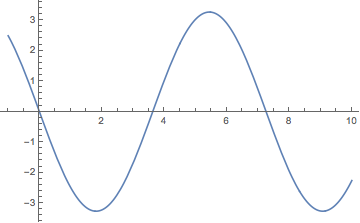
\includegraphics[scale=0.5]{wave1}}
\subfigure[\ ]{
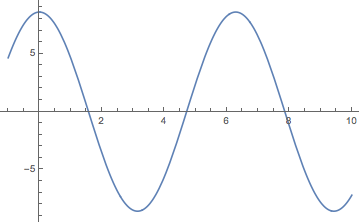
\includegraphics[scale=0.5]{wave2}}
\subfigure[\ ]{
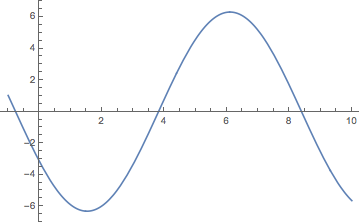
\includegraphics[scale=0.5]{wave3}}
\subfigure[\ ]{
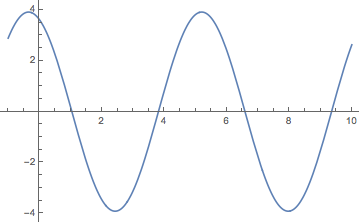
\includegraphics[scale=0.5]{wave4}}
\caption{\protect{\label{oscilador}}  En la figura (a) se muestra la gr\'afica de la funci\'on para $\phi=\frac{\pi}{2},  v_0 = 5,  m=  4,  k=3  $ y $x_0=2.$En la figura (b) se muestra la gr\'afica de la funci\'on para $\phi=0,  v_0 = 10,  m=  41,  k= 1  $ y $x_0=8$.
En la figura (c) se muestra la gr\'afica de la funci\'on para $\phi=\frac{2\pi}{3},  v_0 = 7,  m=  3,  k=\sqrt{2}  $ y $x_0=5.$
En la figura (d) se muestra la gr\'afica de la funci\'on para $\phi=\frac{\pi}{8},  v_0 =  3,  m=  1,  k=\frac{9}{7}  $ y $x_0=\sqrt{13}.$}
\end{figure*}
%
La gr\'afica de la funci\'on (\ref{oscilador-f}) para diferentes valores de $x_0,  k,  m,  \phi$ y $v_0$ puede ver en la figura (\ref{oscilador}).\\
Sus principales caracter\'sticas son las siguientes:
%
\begin{enumerate}
  \item Est\'a confinada entre $x= \pm A$. Esta cantidad se conoce con la amplitud de el movimiento.
  \item El movimiento tiene un periodo $T$ igual a el tiempo transcurrido entre dos puntos equivalentes de la onda.
  \item $\phi$ es la fase de la onda.
  \item $\omega$ es la frecuencia de la onda.
\end{enumerate}
%
\begin{figure*}
\centering
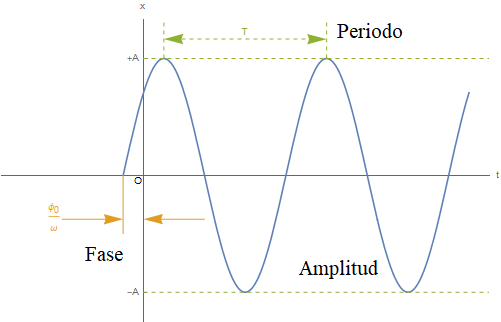
\includegraphics[scale=0.8]{onda}
\caption{\label{onda}  En la gr\'afica se muestran las partes de la onda.  }
\end{figure*}
% 
\'Estas partes se muestran en la figura (\ref{onda}).

%
\section{Superposici\'on de dos vibraciones de la misma frecuencia}
Si tenemos dos vibraciones con la misma frecuencia
%
\begin{eqnarray}
x_1(t)&=& A_1\cos(\omega t + \phi_1), \nonumber\\
x_2(t)&=&A_2\cos(\omega t + \phi_2). \nonumber
\end{eqnarray}
%
Los sumamos y obtenemos
%
\begin{eqnarray}
x(t)= A_1\cos(\omega t + \phi_1) + A_2\cos(\omega t + \phi_2). \nonumber
\end{eqnarray}
%
Podemos suponer que la suma se puede expresar como una s\'ola vibraci\'on. Entonces tenemos
%
\begin{eqnarray}
x(t)= A_1\cos(\omega t + \phi_1) + A_2\cos(\omega t + \phi_2) = A\cos(\omega t + \phi). \nonumber
\end{eqnarray}
%
Hay que encontrar los valores de $A$ ,$\omega$ y $\phi$ para los que se cumple la ecuaci\'on. Usaremos la identidad trigonom\'etrica
%
\begin{eqnarray}
\cos(a+b)= \cos(a) \cos(b) - \sin(a) \sin(b).\label{trig-cos}
\end{eqnarray}
%
Y obtenemos lo siguiente
%
\begin{eqnarray}
A_1\cos(\omega t ) \cos(\phi_1) - A_1\sin(\omega t) \sin(\phi_1) + A_2\cos(\omega t)\cos(\phi_2) \nonumber\\
- A_2\sin(\omega t)\sin(\phi_2)\qquad = A\cos(\omega t)\cos(\phi) - A\sin(\omega t)\sin(\phi). \nonumber
\end{eqnarray}
%
Factorizamos $\cos(\omega t)$ y $\sin(\omega t)$ y obtenemos:
%
\begin{eqnarray}
\cos(\omega t)\left( A_1\cos(\phi_1) + A_2\cos(\phi_2) \right) + \sin (\omega t)\left( A_1\sin(\phi_1) + A_2\sin(\phi_2) \right)\nonumber\\ 
= A\cos(\omega t)\cos(\phi) - A\sin(\omega t)\sin(\phi).\nonumber
\end{eqnarray}
Agrupamos los t\'erminos que tienen $\cos(\omega t)$ y los que tienen $\sin(\omega t)$. Los t\'erminos $\cos(\omega t)$ y $\sin(\omega t)$ se eliminan. Obtenemos:
%
\begin{eqnarray}
A_1\cos(\phi_1) + A_2\cos(\phi_2) &=& A\cos(\phi),\nonumber\\
A_2\sin(\phi_1) + A_2\sin(\phi_2) &=& A\sin(\phi).\nonumber
\end{eqnarray}
%
Elevamos ambos lados de las ecuaciones al cuadrado:
%
\begin{eqnarray}
\left(A_1\cos(\phi_1) + A_2\cos(\phi_2) \right)^2&=& \left(A\cos(\phi)\right)^2, \nonumber\\
\left(A_2\sin(\phi_1) + A_2\sin(\phi_2) \right)^2&=& \left(A\sin(\phi)\right)^2. \nonumber
\end{eqnarray}
%
Obtenemos lo siguiente:
\begin{eqnarray}
A_1^2\cos^2(\phi_1) + 2A_1\cos(\phi_1)A_2\cos(\phi_2)+ A_2^2\cos^2(\phi_2) &=& A^2\cos^2(\phi),\nonumber \\
A_2^2\sin^2(\phi_1) + 2A_2\sin(\phi_1)A_2\sin(\phi_2) + A_2^2\sin^2(\phi_2)&=& A^2\sin^2(\phi).\nonumber
\end{eqnarray}
%
Sumamos ambos t\'erminos y obtenemos
%
\begin{eqnarray}
A_1^2\cos^2(\phi_1) + 2A_1\cos(\phi_1)A_2\cos(\phi_2)+ A_2^2\cos^2(\phi_2) + A_2^2\sin^2(\phi_1) \nonumber \\
+ 2A_2\sin(\phi_1)A_2\sin(\phi_2) + A_2^2\sin^2(\phi_2)\nonumber = A^2\cos^2(\phi) + A^2\sin^2(\phi). \nonumber
\end{eqnarray}
%
Factorizamos t\'erminos y obtenemos lo siguiente
%
\begin{eqnarray}
A_1^2(\cos^2(\phi_1)+\sin^2(\phi_1)) + A_2^2(\cos^2(\phi_2)+\sin^2(\phi_2)) + 2A_1A_2(\cos(\phi_1)\cos(\phi_2)\nonumber \\
\sin(\phi_1)\sin(\phi_2))\nonumber = A^2(\sin^2(\phi)+\cos^2(\phi))\nonumber.
\end{eqnarray}
%
Simplificamos y obtenemos lo siguiente
%
\begin{eqnarray}
A_1^2+A_2^2+2A_1A_2\cos(\phi_1-\phi_2)= A^2. \nonumber
\end{eqnarray}
%
Ahora, para
% 
$$\phi_1=\phi_2$$
%
 tenemos lo siguiente:
\begin{eqnarray}
A_1^2+A_2^2+2A_1A_2\cos(0)&=& A^2,\label{sumavib1}\\
A_1^2+A_2^2+2A_1A_2&=&A^2,\label{sumavib2}\\
(A_1+A_2)^2&=&A^2,\label{sumavib3}\\
A_1+A_2&=&A\label{sumavib4}.
\end{eqnarray}
%
De las ecuaciones (\ref{sumavib1}) - (\ref{sumavib4}) podemos concluir que cuando las vibraciones tienen la misma fase amplitud de la vibraci\'on resultante es la suma de la amplitud de las vibraciones originales. Ahora, cuando 
%
$$\phi_1-\phi_2=\pi$$
%
 tenemos
%
\begin{eqnarray}
A_1^2+A_2^2+2A_1A_2\cos\left(\pi\right)&=& A^2,\label{restavib1}\\
A_1^2+A_2^2-2A_1A_2&=&A^2,\label{restavib2}\\
(A_1-A_2)^2&=&A^2,\label{restavib3}\\
\abs{A_1-A_2}&=&A\label{restavib4}.
\end{eqnarray}
%
Para el \'angulo de la fase de la vibraci\'on resultante tenemos lo siguiente:
%
\begin{eqnarray}
\tan(\phi)=\frac{A\sin(\phi)}{A\cos(\phi)}=\frac{A_1\sin(\phi_1)+A_2\sin(\phi_2)}{A_1\cos(\phi_1)+A_2\cos(\phi_2)}\nonumber
\end{eqnarray}
%
\animategraphics[label=anim,autoplay,controls]
{12}{fig/anim}{00}{85}
%
En la figura (\ref{anim}) se puede apreciar el comportamiento descrito.
%
De las ecuaciones (\ref{restavib1})-(\ref{restavib4}) concluimos que, cuando la diferencia de las fases es $\pi$ entonces la amplitud de la vibraci\'on resultante es igual a la resta de las amplitudes originales. En particular, si además las amplitudes son iguales la amplitud resultante es igual a cero. 
\section{Superposici\'on de dos vibraciones de diferente frecuencia}
%
Dadas dos vibraciones con diferente frecuencia, la misma fase  y amplitud
%
\begin{eqnarray}
x_1(t)&=& A\cos(\omega_1 t),\nonumber\\
x_2(t)&=&A\cos(\omega_2 t),\nonumber.
\end{eqnarray}
%
Al sumar estas funciones encontramos 
%
\begin{eqnarray}
x(t)=A\left(  \cos(\omega_1 t)+\cos(\omega_2 t)\right).
\label{resultrig}
\end{eqnarray}
%
Tomando en cuenta la identidad 
%
\begin{eqnarray}
\cos(a) \cos(b)=\frac{1}{2} \left( \cos(a+b)+ \cos(a-b)\right),
\end{eqnarray}
%
entonces (\ref{resultrig}) se transforma en
%
\begin{eqnarray}
x(t)= 2A\cos \left( \frac{\omega_1  +\omega_2}{2} t \right) \cos\left( \frac{\omega_1 t-\omega_2 t}{2} t \right) \nonumber
\end{eqnarray}
% 
\begin{figure*}
\centering
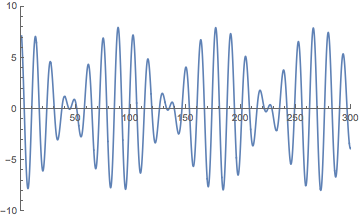
\includegraphics[scale=0.8]{fig/2diferentefrecuencia}
\label{fig:dosdiferentefrecuencia}
\caption{Superposici\'on de dos oscilaciones con diferente frecuencia.  }
\end{figure*}
%
En la gr\'afica (\ref{fig:dosdiferentefrecuencia}) se aprecia el comportamiento de la Superposici\'on de dos vibraciones con diferente frecuencia.
\section{El oscilador con dos masas} 
\begin{figure*}
\centering

\includegraphics[scale=0.8]{fig/dosmasas}
\caption{\label{dosmasas}  Dos masas sujetas por tres resortes.  }
\end{figure*}
Veamos ahora que sucede cuando hay dos masas sujetas entre tres resortes como se muestra en la figura (\ref{dosmasas}). Sean $x_1$ y $x_2$ los desplazamientos de las masas desde sus respectivas posiciones de equilibrio (cuando los resortes no est\'an estirados), $k$ la constante de los resortes de los extremos y $\kappa$ la constante del resorte de enmedio. El resorte de enmedio est\'a estirado (o comprimido) por $x_2-x_1$. Entonces, las ecuaciones $F=ma$ para las dos masas son:
%
\begin{eqnarray}
m\ddot x_1 &=& -kx_1-\kappa(x_1-x_2),\label{dosmasas1}\\
m\ddot x_2 &=& -kx_2-\kappa(x_2-x_1).\label{dosmasas2}
\end{eqnarray}
%
Suponemos las soluciones de la forma 
%
\begin{eqnarray}
x_1(t)&=&A_1e^{i\omega t},\\
x_2(t)&=&A_2e^{i\omega t}.
\end{eqnarray}
%
Es conveniente escribirlas de la siguiente forma
%
\[\begin{pmatrix}
x_1(t)\\
x_2(t)
\end{pmatrix} = \begin{pmatrix}
A_1\\
A_2
\end{pmatrix} e^{i\omega t}\]
%
Sustituimos las soluciones en las ecuaciones (\ref{dosmasas1}-\ref{dosmasas2}), cancelamos el t\'ermino $e^{i\omega t}$ y obtenemos lo siguiente:
%
\begin{eqnarray}
-m\omega ^2A_1 &=& -kA_1 - \kappa(A_1-A_2),\\
-m\omega ^2A_2 &=& -kA_2 - \kappa(A_1-A_2).
\end{eqnarray}
%
En forma matricial tenemos
%
\begin{eqnarray}
\begin{pmatrix}
-m\omega ^2 + k + \kappa & -\kappa\\
-\kappa & -m\omega ^2 + k + \kappa
\end{pmatrix} \begin{pmatrix}
A_1\\
A_2
\end{pmatrix} = \begin{pmatrix}
0\\
0
\end{pmatrix}.\label{matricial}
\end{eqnarray}
%
Una soluci\'on trivial viene de multiplicar el sistema por la inversa de la matriz que contiene los t\'erminos $\omega$, $\kappa$ y $k$ lo cual conduce a 
%
\[\begin{pmatrix}
A_1\\
A_2\end{pmatrix}= \begin{pmatrix}
0\\
0\end{pmatrix}.\]
%
Una soluci\'on no trivial donde hay movimiento es cuando la inversa de la matriz no existe. Tomamos
%
\begin{eqnarray}
A^{-1} = \frac{(adj(A))^t}{Det(A)}.
\end{eqnarray}
%
Es decir, la matriz inversa no existe cuando el determinante de la matriz es igual a cero.
%
Hacemos el determinante igual a cero
%
\[\begin{vmatrix}
-m\omega ^2 + k + \kappa & -\kappa\\
-\kappa & -m\omega ^2 + k + \kappa
\end{vmatrix} = 0,\]
%
nos da la siguiente ecuaci\'on.
%
\begin{eqnarray}
(-m\omega ^2 + k + \kappa)^2 - \kappa ^2 = 0.
\end{eqnarray}
%
De ah\'i obtenemos
%
\begin{eqnarray}
-m \omega ^2 + k + \kappa =\pm \kappa .
\end{eqnarray}
%
Entonces tenemos las siguientes soluciones
%
\begin{eqnarray}
\omega ^2 &=& \frac{k}{m},\\
\omega ^2 &=& \frac{k+ 2 \kappa}{m}.
\end{eqnarray}
%
O sea
%
\begin{eqnarray}
\omega &=& \pm \sqrt{\frac{k}{m}},\\
\omega &=& \sqrt{\frac{k+ 2 \kappa}{m}}
\end{eqnarray}
%
En el caso en que $\omega ^2 =\frac{k}{m}$ sustituimos en la ecuaci\'on \ref{matricial} y obtenemos lo siguiente
%
\[\kappa \begin{pmatrix}
1 & -1\\
-1 & 1
\end{pmatrix} \begin{pmatrix}
A_1\\
A_2
\end{pmatrix} = \begin{pmatrix}
0\\
0
\end{pmatrix}.\]
%
Ambos renglones nos dan el mismo resultado, entonces $A_1 = A_2$, o lo que es lo mismo $(A_1, A_2)$ es proporcional al vector $(1,1)$.\\
Para el caso en que $\omega ^2 = \frac{k + 2\kappa}{m}$ tenemos lo siguiente
%
\[\kappa \begin{pmatrix}
-1 & -1\\
-1 & -1
\end{pmatrix} \begin{pmatrix}
A_1\\
A_2
\end{pmatrix} = \begin{pmatrix}
0\\
0
\end{pmatrix}.\]
%
De ambos renglones obtenemos $A_1 = -A_2$. Entonces $(A_1, A_2)$ es proporcional al vector $(1,-1)$. Tomando $\omega_1 \equiv  \sqrt{\frac{k}{m}}$ y $\omega_2 \equiv \sqrt{\frac{k + 2\kappa}{m}}$ escribimos la solucion general como la suma de las cuatro soluciones encontradas. La soluci\'on est\'a
 dada por:
 %
\[\begin{pmatrix}
x_1(t)\\
x_2(t)
\end{pmatrix} = C_1 \begin{pmatrix}
1 \\
1
\end{pmatrix}e^{i\omega_1 t} + C_2 \begin{pmatrix}
1\\
1
\end{pmatrix}e^{-i\omega_2 t}+ C_3 \begin{pmatrix}
1\\
-1
\end{pmatrix}e^{i\omega_1 t}+ C_4 \begin{pmatrix}
1\\
-1
\end{pmatrix}e^{-i\omega_2 t} .\]
%
S\'olo la parte real tiene una interpretaci\'on f\'isica, entonces $C_1 = C_2 \equiv \frac{A_1}{2}e^{i\omega_1}$ y $C_3 = C_4 \equiv \frac{A_2}{2}e^{i\omega_2}$. Entonces obtenemos:\\
%
 \[\begin{pmatrix}
x_1(t)\\
x_2(t)
\end{pmatrix} = A_1 \begin{pmatrix}
1 \\
1
\end{pmatrix}\cos(\omega_1 t + \phi_1) + A_2 \begin{pmatrix}
1\\
-1
\end{pmatrix}\cos(\omega_2 t + \phi2).\]
%
Es decir
%
\begin{eqnarray}
x_1(t)&=&A_1 \cos(\omega_1 t + \phi_1) + A_2 \cos(\omega_2t+\phi_2)\nonumber, \\
x_2(t)&=&A_1 \cos(\omega_1 t + \phi_1) - A_2 \cos(\omega_2t+\phi_2)\label{sol2masas}.
\end{eqnarray}
% 
\section{Modos Normales}
Ahora, si $A_2 = 0$ en la ecuaci\'on (\ref{sol2masas}) tenemos que
%
\begin{eqnarray}
x_1(t)=x_2(t)=A_1\cos(\omega_1 t + \phi_1).
\end{eqnarray}
%
Entonces ambas masas se mueven exactamente de la misma manera. Ambas a la izquierda, ambas a la derecha, etc. Esto es consistente con el hecho de que $\omega_1 = \sqrt{\frac{k}{m}}$, independiente de $\kappa$. Este movimiento, en el que las dos masas se mueven con la misma frecuecia es llamado modo normal. Para especificar un modo normal hace falta especificar su frecuencia y tambi\'en sus amplitudes relativas. En este caso, el modo tiene frecuencia $\omega_1 = \frac{k}{m}$ y las amplitudes son iguales.\\
El otro caso, cuando $A_1=0$ en la ecuacion (\ref{sol2masas}) nos da
%
\begin{eqnarray}
x_1(t)=-x_2(t)=A_2\cos(\omega_2 t + \phi_2).
\end{eqnarray}
%
En este caso las masas se mueven en direcci\'on opuesta. La frecuencia ahora es $\omega_1 = \sqrt{\frac{k+2\kappa}{m}}$. En este caso la frecuencia $\omega_1$ es menor que $\omega_2$ ya que en este caso el resorte de enmedio est\'a estirado o comprimido participa en la fuerza restauradora. 
%
\section{Oscilador con tres masas}
\begin{figure*}
\centering

\includegraphics[scale=0.5]{fig/tresmasas}
\caption{\label{Tresmasas}  Tres masas sujetas con resortes.  }
\end{figure*}
%
En este caso $x_1$, $x_2$ y $x_3$ son los desplazamientos de las tres masas y asumimos que la constante $k$ es igual para todos los resortes. Entonces tenemos las ecuaciones:
%
\begin{eqnarray}
m\ddot x_1 &=& -kx_1-k(x_1-x_2),\label{tresmasas1}\\
m\ddot x_2 &=& -k(x_2-x_1)-k(x_2-x_3)\label{tresmasas2},\\
m\ddot x_3 &=& -k(x_3-x_2)-kx_3.\label{tresmasas3}
\end{eqnarray}
%
Estamos buscando una soluci\'on de la forma:
%
\[\begin{pmatrix}
x_1(t)\\
x_2(t)\\
x_3(t)
\end{pmatrix} = \begin{pmatrix}
A_1 \\
A_2 \\
A_3 
\end{pmatrix}e^{i\omega t}.\]
%
Sustituimos en las ecuaciones (\ref{tresmasas1}-\ref{tresmasas3}) y obtenemos lo siguiente:
%
\begin{eqnarray}\begin{pmatrix}
-\omega ^2+2\omega_0^2 & -\omega ^2 & 0\\
-\omega_0^2 & -\omega ^2+2\omega_0^2 & -\omega_0^2\\
0 & -\omega_0^2 & -\omega ^2+2\omega_0^2
\end{pmatrix} \begin{pmatrix}
A_1 \\
A_2 \\
A_3 
\end{pmatrix}= \begin{pmatrix}
0 \\
0 \\
0 
\end{pmatrix}\label{tresmasaseq}, 
\end{eqnarray}
%
donde $\omega_0^2 = \frac{k}{m}$. Como en el caso donde tenemos dos masas, una soluci\'on no trivial existe cuando el determinante de la matriz es cero. Haciendo el determinante igual a cero obtenemos:
%
\begin{eqnarray}
(-\omega^2 +2\omega_0^2)((-\omega^2+2\omega_0^2)^2 -\omega_0^4)+\omega_0^2(-\omega_0^2(-\omega^2+2\omega_0^2))&=&0,\\
\implies (-\omega^2+2\omega_0^2)(\omega^4-4\omega_0^2\omega^2+2\omega_0^4)&=&0,
\end{eqnarray}
%
la cual es una ecuaci\'on cuadratica para $\omega$. Usando la f\'ormula cuadr\'atica obtenemos:
$$\omega^2=2\omega_0^2 \qquad y \qquad \omega^2 = (2 \pm \sqrt{2})\omega_0.$$
Sustituyendo en la ecuaci\'on (\ref{tresmasaseq}) obtenemos los tres modos normales:
%
\begin{eqnarray}
\omega = \pm\sqrt{2}\omega_0 \implies \begin{pmatrix}
A_1 \\
A_2 \\
A_3 
\end{pmatrix} &\propto& \begin{pmatrix}
1 \\
0 \\
-1 
\end{pmatrix},\\
\omega = \pm\sqrt{2+\sqrt{2}}\omega_0 \implies \begin{pmatrix}
A_1 \\
A_2 \\
A_3 
\end{pmatrix} &\propto& \begin{pmatrix}
1 \\
-\sqrt{2} \\
-1 
\end{pmatrix},\\
\omega = \pm\sqrt{2-\sqrt{2}}\omega_0 \implies \begin{pmatrix}
A_1 \\
A_2 \\
A_3 
\end{pmatrix} &\propto& \begin{pmatrix}
1 \\
\sqrt{2} \\
-1 
\end{pmatrix}.   
\end{eqnarray}
%
Tomando de nuevo la parte real obtenemos lo siguiente
\begin{eqnarray}
\begin{pmatrix}
x_1\\
x_2 \\
x_3 
\end{pmatrix} = A_1 \begin{pmatrix}
1 \\
0 \\
-1 
\end{pmatrix}\cos\left(\sqrt{2}\omega_0 t + \phi_1\right) +  A_2 \begin{pmatrix}
1 \\
-\sqrt{2} \\
-1 
\end{pmatrix}\cos\left(\sqrt{2+\sqrt{2}}\omega_0 t + \phi_2\right) \nonumber\\+ 
A_3 \begin{pmatrix}
1 \\
\sqrt{2} \\
1 
\end{pmatrix}\cos\left(\sqrt{2-\sqrt{2}}\omega_0 t + \phi_3\right) \nonumber. 
\end{eqnarray}
%
\section{Oscilador con $N$ masas}
Ahora consideremos el caso con n masas entre dos muros unidas con resortes. Las masas son todas iguales a $m$ y las constantes de resorte son iguales a k y los desplazamientos de sus masas iguales a $x_1,x_2,\dots,x_n$. La fuerza en ela en\'esima masa es: 
%
\begin{eqnarray}
F_n = -k(x_n - x_{n-1}) - k(x_n-x_{n+1})= kx_{n-1} - 2kx_n+kx_{n+1}.
\end{eqnarray}
%
Entonces lo que obtenemos es una colecci\'on de ecuaciones parecidas a esta
%
\begin{eqnarray}
m \ddot x_n = kx_{n-1}-2kx_n+kx_{n+1}\label{enesima}.
\end{eqnarray}
%
Juntamos todas en la ecuaci\'on matricial y obtenemos:
%
\begin{eqnarray}m\frac{d^2}{dt^2}
\begin{pmatrix}
\vdots\\
x_{n-1}\\
x_n\\
x_{n+1} \\
\vdots
\end{pmatrix} = \begin{pmatrix}
 & & \vdots \\
\cdots & k & -2k & k\\
 & & k & -2k & k\\
  & & & k & -2k & k & \cdots\\
  & & & & \vdots \\
\end{pmatrix}\begin{pmatrix}
\vdots\\
x_{n-1}\\
x_n\\
x_{n+1} \\
\vdots
\end{pmatrix}
\end{eqnarray}
%
Buscamos soluciones de la forma
%
\begin{eqnarray}
\begin{pmatrix}
\vdots\\
x_{n-1}\\
x_n\\
x_{n+1} \\
\vdots
\end{pmatrix} = \begin{pmatrix}
\vdots\\
A_{n-1}\\
A_n\\
A_{n+1} \\
\vdots
\end{pmatrix}e^{i\omega t},
\end{eqnarray}
%
solo que en lugar de usar el m\'etodo del determinante como lo hicimos para los casos en que $n=2$ y $n=3$ masas analizaremos las ecuaciones individualmente. Consideremos la en\'esima ecuaci\'on. Tomamos $x_n(t) = A_n e^{i\omega t}$, derivamos y sustituimos en la ecuaci\'on (\ref{enesima}) y obtenemos:
%
\begin{eqnarray}
-\omega^2 A_n &=& \omega_0^2(A_{n-1}-2A_n+A_{n+1}),\\
\implies \frac{A_{n-1}+A_{n+1}}{A_n} &=& \frac{2\omega_0^2-\omega^2}{\omega_0^2}\label{eqnthmasas}.
\end{eqnarray}
%
Donde $\omega_0 = \sqrt{\frac{k}{m}}$. La ecuaci\'on se debe cumplir para todos los valores de n desde $1$ hasta $N$, entonces tenemos $N$ ecuaciones de esta forma. Para alg\'un modo con una frecuencia $\omega$ la cantidad $\frac{2\omega_0^2-\omega^2}{\omega_0^2}$ es una constante independiente de $n$. Entonces la relaci\'on $\frac{A_{n-1}+A_{n+1}}{A_n}$ en el lado izquierdo de (\ref{eqnthmasas}) tambi\'en es una constante independiente de $n$. Entonces, para 3 $A's$ adyacentes conocidas entonces el valor del cociente se puede determinar f\'acilmente. De igual forma, para 3 $A's$ adyacentes y $\omega$ conocidas entonces se puede determinar el valor de $\frac{2\omega_0^2-\omega^2}{\omega_0^2}$. El problema es encontrar la forma que tienen que tomar las $A's$ para que el cociente $\frac{A_{n-1}+A_{n+1}}{A_n}$ sea independiente de $n$.
%
\begin{proposition}
Si $\omega < 2\omega_0$ entonces cualquier conjunto de $A_n's$ que satisfacen el sistema de $N$ ecuaciones (\ref{eqnthmasas}) puede eser escrito como:
%
\begin{eqnarray}
A_n=B\cos(n\theta)+C\sin(n\theta).\label{inductiva}
\end{eqnarray}
%
Para ciertos valores de $B$, $C$ y $\theta$. 
%
\end{proposition}
%
\begin{proof}
Comenzamos por definir
%
\begin{eqnarray}
\cos(\theta) \equiv \frac{A_{n-1}+A_{n+1}}{2A_n}.\label{costheta}
\end{eqnarray}
%
Si nos fijamos en alg\'un modo normal con frecuencia $\omega$, entonces por la ecuaci\'on (\ref{eqnthmasas}) una definici\'on equivalende de $\theta$ es 
%
\begin{eqnarray}
2\cos(\theta) \equiv \frac{2\omega_0^2-\omega^2}{\omega_0^2}.\label{2costheta}
\end{eqnarray}
%
Estas definiciones s\'olo est\'an definidas si producen un valor de $\cos(\theta)$ que satisface $\abs{\cos(\theta)}\leq 1$. Esta condici\'on es equivalente a que $\omega$ debe satisfacer $-2\omega_0 < \omega < 2\omega_0$. De la ecuaci\'on (\ref{eqnthmasas}) podemos ver que si conocemos dos de las $A's$ podemos determinar un valor de $\omega$. Supongamos que conocemos $A_0$ y $A_1$. El resto de las $A's$ puede ser determinado como sigue. Se define $B$ como:  
%
\begin{eqnarray}
A_0 \equiv B\cos(1\cdot \theta) + C\sin (0 \cdot \theta) \implies A_0\equiv B.
\end{eqnarray}
%
Una vez que $B$ ha sido definido se define $C$ como
%
\begin{eqnarray}
A_1 \equiv B\cos(1\cdot \theta) + C \sin(1\cdot\theta) \implies A_1\equiv B \cos(\theta)+C\sin(\theta).
\end{eqnarray}
%
Para cualquier $A_0$ y $A_1$ estas ecuaciones determinan de manera \'unica $B$ y $C$, $\theta$ ya estaba definida por $\omega$. Por costrucci\'on, estas definiciones se cumplen para $n=0$ y $n=1$. Se demostrar\'a por inducci\'on que se cumple para toda $n$.\\
Tomemos la hip\'otesis inductiva (\ref{inductiva}) y hagamos los c\'alculos para $A_{n+1}$:
%
\begin{eqnarray}
A_{n+1}&=&(2\cos(\theta))A_n-A_{n-1},\\
A_{n+1}&=&2\cos(\theta)(B\cos(n\theta)+C\sin(n\theta))-(B\cos(n-1)\theta\\
&+&C\sin(n-1)\theta),\nonumber\\
A_{n+1}&=&B(2\cos (n\theta)\cos(\theta)-(\cos(n\theta)\cos(\theta))+\sin(n\theta\sin(\theta)))\\
&+&C(2\sin(n\theta)\cos(\theta)-(\sin(n\theta)\cos(\theta))-\cos(n\theta) \sin(\theta))\nonumber,\\
&=&B(\cos(n\theta)\cos(\theta) -\sin(n\theta)\sin(\theta))+C(\sin(n\theta)\cos(\theta)\nonumber\\
&+& \cos(n\theta)\sin(\theta)). \\
&=&B\cos ((n+1)\theta) + C\sin((n+1)\theta).
\end{eqnarray}
%
Que es justo la expresi\'on esperada para $A_{n+1}$ por lo tanto se cumple para un n\'umero infinito de masas en ambas direcciones.
\end{proof}
%
Lo que esto nos dice es que hemos encontrado una soluci\'on de la forma
%
\begin{eqnarray}
x_n(t)=A_ne^{i\omega t} = (B\cos(n\theta)+C\sin\theta)e^{i\omega t}\label{soln1}.
\end{eqnarray}
%
Esto asumiendo que $\omega$ es positiva. Sin embargo hay que recordar que 
%
x\begin{eqnarray}
x_n(t)=A_ne^{-i\omega t} = (D\cos(n\theta)+E\sin\theta)e^{-i\omega t}\label{soln2},
\end{eqnarray}
%
tambi\'en es soluci\'on. Como las ecuaciones del tipo (\ref{enesima}) son lineales la suma de las soluciones tambi\'en es soluci\'on. Entonces la soluci\'on m\'as general es la suma de las soluciones (\ref{soln1}) y (\ref{soln2}). \\
De nuevo, las soluciones tienen que ser reales. Esto implica que (\ref{soln1}) y (\ref{soln2}) deben ser ser el conjugado la una de la otra. Y como esto debe cumplirse para todos los valores de $n$, $B$ y $D$ deben ser conjugados complejos al igual que $C$ y $E$. Entonces definimos $B=D^*\equiv \frac{F}{2}e^{i\beta}$ y $C=E^*\equiv \frac{G}{2}e^{i\gamma}$. La suma de las dos soluciones se convierte en
%
\begin{eqnarray}
x_n(t)=F\cos(n\theta)\cos(\omega t + \beta) + G\sin(n\theta) \cos(\omega t + \gamma)
\end{eqnarray}
%
Usando la f\'ormula del coseno de una suma podemos reescribirla como:
%
\begin{eqnarray}
x_n(t)=C_1 \cos(n\theta) \cos(\omega t) + C_2 \cos (n \theta)\sin(\omega t) + C_3 \sin(n\theta)\cos(\omega t) \nonumber
\\+ C_4 \sin(n\theta)\sin(\omega t),
\end{eqnarray}
%
donde $\theta$ est\'a determinado por
%
\begin{eqnarray}
\theta \equiv \cos ^{-1} \left(\frac{2\omega_0^2-\omega^2}{2 \omega_0^2}\right)
\end{eqnarray}
%
\section{$N \to \infty$ y la ecuaci\'on de onda}
Ahora consideremos el caso $N \to \infty$ l\'imite para el arreglo de masas y resortes. Lo que obtenemos es un sistema continuo. Ahora $x$ representar\'a las posiciones de las masas en reposo y $\xi$ el desplazamiento de las masas, de esta forma $\xi_n$ es el desplazamiento de la en\'esima masa. Las $x's$ son constantes, s\'olamente son para nombrar las posiciones de quilibrio, que son fijas. La posici\'on de la en\'esima masa es $x_n + \xi_n$ pero s\'olo la parte $\xi_n$ aparece en la ecuaci\'on $F=ma$ ya que s\'olo $\xi_n$ contribuye a la aceleraci\'on. Escribiremos la funci\'on del deplazamiento como $\xi(x_n)$ y por ahora no escribiremos la dependencia temporal.\\
Sea $\Delta x \equiv x_n - x_{n-1}$ el espacio igual entre las posiciones de equilibrio de todas las masas. Entonces, la ecuaci\'on $F=ma$ se convierte en:
%
\begin{eqnarray}
m\ddot \xi_n &=& k\xi_{n-1}-2k\xi_n + k\xi_{n+1}\\
\implies m\ddot \xi(x_n) &=& k\xi(x_n-\Delta x)-2k\xi(x_n)+ k\xi(x_n + \Delta x),\\
\implies m\ddot \xi(x_n) &=& k\xi(x-\Delta x)-2k\xi(x)+ k\xi(x + \Delta x).
\end{eqnarray}
%
El primer paso es regresarlo a una ecuaci\'on de la forma $F=ma$. Entonces tenemos:
%
\begin{eqnarray}
m\frac{d^2\xi(x)}{dt^2}&=&k\left[(\xi (x+\Delta x)-\xi(x))-(\xi(x)-\xi(x-\Delta x)) \right]\\
\implies \frac{m}{\Delta x}\frac{d^2\xi(x)}{dt^2}&=&k\Delta x\left(\frac{\frac{\xi(x+\Delta x)-\xi(x)}{\Delta x}-\frac{\xi(x)-\xi(x-\Delta x)}{\Delta x}}{\Delta x} \right)
\end{eqnarray}
%
Entonces usamos las definiciones de 1er y 2a derivada para obtener:
%
\begin{eqnarray}
\frac{m}{\Delta x}\frac{d^2\xi(x)}{dt^2} &=&(k\Delta x)\frac{\xi'(x)-\xi'(x-\Delta x)}{\Delta x},\\
&=&(k\Delta x)\xi''(x),
\end{eqnarray}
%
donde $\frac{m}{\Delta x}$ es conocida como la densidad de masa $\rho$ y $(k\Delta x)$ es conocida como el m\'odulo el\'astico $E$. Entonces la ecuaci\'on se reescribe como:
%
\begin{eqnarray}
\rho \frac{d^2 \xi(x)}{dt^2}=E\xi''(x)
\end{eqnarray}
%
Como $\xi$ es una funci\'on de $x$ y $t$ procedemos a escribir:
%
\begin{eqnarray}
\rho \frac{\partial^2 \xi(x,t)}{\partial t^2}=E\frac{\partial^2 \xi(x,t)}{\partial t^2}.\label{eqonda}
\end{eqnarray}
%
Que es conocida como la ecuaci\'on de onda. Para resolver la ecuaci\'on de onda podemos retomar la estrategia del caso del oscilador con $N$ masas. Suponemos que la soluci\'on es del tipo:
\begin{eqnarray}
\begin{pmatrix}
\vdots\\
\xi_{n-1}\\
\xi_n\\
\xi_{n+1}\\ 
\vdots
\end{pmatrix}=\begin{pmatrix}
\vdots\\
a_{n-1}\\
a_n\\
a_{n+1}\\
\vdots
\end{pmatrix}e^{i\omega t}.
\end{eqnarray}
%
Si re etiquetamos $\xi_n \rightarrow \xi(x_n,t) \rightarrow \xi(x,t)$ y $a_n \rightarrow a(x_n) \rightarrow a(x)$ podemos reescribir nuestra suposici\'on como:
%
\begin{eqnarray}
\xi(x,t)=a(x)e^{i\omega t}\label{supon}.
\end{eqnarray}
%
Esto es, de hecho, un conjunto infinito de ecuaciones (una para cada x). La ecuaci\'on $a(x)$ da las amplitudes de las masas. Entonces, sustituyendo en la expresi\'on (\ref{eqonda}) obtenemos lo siguiente: 
%
\begin{eqnarray}
\rho \frac{\partial ^2}{\partial t^2}(a(x)e^{i\omega t})&=&E\frac{\partial^2}{\partial x^2}(a(x)e^{i\omega t}),\\
\implies -\omega^2\rho a(x) &=& E\frac{d^2}{dx^2}(a(x)),\\
\implies \frac{d^2}{dx^2}(a(x)) &=& -\frac{\omega^2\rho}{E}(a(x)).\label{solwave}
\end{eqnarray}
%
En la ecuaci\'on (\ref{solwave}) lo que tenemos es la ecuaci\'on de un oscilador arm\'onico 
$$a(x)=Ae^{\pm ik x}$$ 
con
%
\begin{eqnarray}
k\equiv \omega \sqrt{\frac{\rho}{E}}, \label{konda}
\end{eqnarray}
%
y se conoce a $k$ como el n\'umero de onda. La interpretaci\'on f\'isica del n\'umero k es la siguiente. Si $\lambda$ es la longitud de onda, entonces el exponente $kx$ en la ecuaci\'on (\ref{konda}) incremente $2\pi$ cada que $x$ incrementa $\lambda$.Entonces tenemos:
%
\begin{eqnarray}
k\lambda = 2\pi \implies k=\frac{2\pi}{\lambda}.
\end{eqnarray}
%
Entonces $k$ es igual al numero de radianes de oscilaciones espaciales que caben en una unidad de longitud. Usando entonces (\ref{konda}) en la soluci\'on la ecuaci\'on (\ref{supon}) se convierte en:
%
\begin{eqnarray}
\xi(x,t)=a(x)e^{i\omega t} = Ae^{(\pm kx + \omega t)}.
\end{eqnarray}
%
\section{El principio de Hamilton}
%
Para describir las interacciones entre part\'iculas se emplean los conceptos de fuerza y energ\'ia potencial. En coordenadas cartesianas la energ\'ia potencial es igual al gradiente de la fuerza cambiado de signo, para una part\'icula se obtiene:
%
\begin{eqnarray}
F_x=-\frac{\partial U}{\partial x}, F_y=-\frac{\partial U}{\partial y}, F_z=-\frac{\partial U}{\partial z},
\end{eqnarray}
%
donde las $F_k$ son las componentes de la fuerza y $U$ es la energ\'ia potenial a veces llamada simplemente \textit{potencial}. $U$ es muy impoprtante por que contiene toda la informaci\'on del sistema. De modo que hayar $U$ equivale a determinar el modelo f\'isico del sistema. Cuando U no depende expl\'icitamente del tiempo se conserva la energ\'ia total que vale la suma de la cin\'etica y la potencial. En este caso se acostumbra llamar fuerzas conservativas a aquellas que se deducen de un potencial. El principio de Hamilton dice que existe una funci\'on potencial para todo sistema ideal y explica como, a partir de ella, se puede obtener su ecuaci\'on de movimiento. 
%
El principio de Hamilton dice: A todo sistema ideal con $n$ grados de libertad con coordenadas $q_1, q_2, \dots , q_n$ lel corresponde una funci\'on $U(q,\dot q, t)$ llamada el potencial, que describe las interacciones, caracteriza y determina el movimiento de la forma siguiente:\\

Cuando el sistema va desde la configuraci\'on $q_k^{(1)}$ en $t=t_1$ hasta la $q_k^{(2)}$ en $t=t_2$, lo hace de modo que la llamada integral de acci\'on S,
%
\begin{eqnarray}
S=\int_{t_1}^{t_2} \left(T(q,\dot q, t)-U(q,\dot q, t)\right)dt,
\end{eqnarray}
%
donde T es la energ\'ia cin\'etica, toma un valor estacionario.\\
%
Definiendo el Lagrangiano o funci\'on Lagrangiana como 
%
\begin{eqnarray}
L(q,\dot q, t)=T(q,\dot q, t)-U(q,\dot q, t),
\end{eqnarray}
%
Se puede escribir la integral de acci\'on como 
%
\begin{eqnarray}
S=\int_{t_1}^{t_2} L(q,\dot q, t)dt,
\end{eqnarray}
%
esto implica que se deben cumplir las ecuaciones de Euler-Lagrange. 
%
\begin{eqnarray}
\frac{d}{dt}\frac{\partial L}{\partial \dot q_k}-\frac{\partial L}{\partial q_k}=0 \qquad k=1,2,\dots ,n, \label{euler-lagrange}
\end{eqnarray}
%
y son entonces las ecuaciones del sistema. \\
%
Como $L$ depende de $q_k$ y $\dot q_k$ entonces (\ref{euler-lagrange}) es un conjunto de $n$ ecuaciones de segundo orden en el que, si la matriz
%
\begin{eqnarray}
L_{ij}=\frac{\partial^2 L}{\partial \dot q_i \partial \dot q_j}
\end{eqnarray}
%
es regular y tiene inversa, popr tanto es posible despejar las aceleraciones que son funciones de las coordenadas y las velocidades. \\
Generalizando se definen las fuerzas omo $F_k$ como las derivadas de potencial respecto a las coordenadas cambiadas de signo, es decir
%
\begin{eqnarray}
F_k= \frac{d}{dt}\frac{\partial U}{\partial \dot q_k},
\end{eqnarray}
%
lo que permite escribir las ecuacione de Lagrange de una forma un poco distinta
%
\begin{eqnarray}
F_k= \frac{d}{dt}\frac{\partial T}{\partial \dot q_k}-\frac{\partial t}{\partial q_k}
\end{eqnarray}
%
\section{La energ\'ia del sistema Lagrangiano}
%
Consideremos ahora un sistema con Lagrangiano
%
\begin{eqnarray}
L= \frac{1}{2}\sum_{i,j}M_{ij}(q)\dot q_i\dot q_j-U(q),
\end{eqnarray}
%
que tiene un punto de equilibrio en $q_i = q_{0i}$. Esto significa que $U(q)$ toma un valor estacionario en $q_{0i}$ y que sus derivadas parciales se anulan all\'i $$\frac{\partial U(q_0)}{\partial q_i}=0$$ por lo que
%
\begin{eqnarray}
U=U(q_0)+\frac{1}{2}\sum_{i,j}\frac{\partial^2 U(q_0)}{\partial q_i \partial q_j}(q_i - q_{0i})(q_j-q_{0j})+O[(q_i-q_{0i})^3]
\end{eqnarray}
%
Si el sistema se aleja un poco de la posici\'on de equilibrio, las cantidades $\dot q_k(t) =  q_k(t)-q_{0k}$, tendr\'an valores pequeños. En ese caso, la primera aproximaci\'on se obtiene despreciando los valores cuadr\'aticos, c\'ubicos, etc en $q_i$ y $\dot q_k$ y conservando s\'olo los lineales.\\
Como la deducci\'on de las ecuaciones desde el Lagrangiano incluye los valores $\frac{\partial L}{\partial q_k} , \frac{\partial L}{\partial \dot q_k}$ eso equivale a tomar s\'olo los t\'erminos de segundo grado en $L$. Entonces, para estudiar las oscilaciones pequeñas en torno a $q_i = 0$ hay que considerar la parte cuadr\'atica del Lagrangiano.
%
\begin{eqnarray}
L=\frac{1}{2}\sum_{i,j}M_{i,j}\dot q_i \dot q_j - \frac{1}{2}\sum_{i,j}K_{i,j}\dot q_i \dot q_j\label{quadlag}
\end{eqnarray}
%
donde $$M_{i,j}=M_{i,j}(0) \qquad y \qquad K_{i,j}= \frac{\partial U(0)}{\partial q_i \partial q_j}$$.\\
La ecuaci\'on de movimiento que se deduce de (\ref{quadlag}) es 
%
\begin{eqnarray}
L=\sum_{j}M_{i,j}\ddot q_j + K_{i,j} q_j,
\end{eqnarray}
%
que se puede escribir en notaci\'on vectorial como
%
\begin{eqnarray}
\textbf{M $\ddot q$ } + \textbf{K q} = 0.
\end{eqnarray}
%
En este caso existen n modos normales de oscilaci\'on, uno por cada grado de libertad, y se obtienen resolviendo un problema de valores propios. Sea el modo $k$-\'esimo
%
\begin{eqnarray}
q=A_k \cos (\omega_kt + \delta_k)
\end{eqnarray}
%
Sustituyendo en (\ref{quadlag}) se obtiene 
%
\begin{eqnarray}
\omega_k^2 MA_k=KA_k \label{lageig},
\end{eqnarray}
%
lo que produce un problema de valores propios. Como (\ref{lageig}) es un sistema homog\'eneo de ecuaciones s\'olo tiene soluci\'on si el determinante se anula, es decir si
%
\begin{eqnarray}
det\left(\textbf(K)-\omega_k^2\textbf(M)\right)=0
\end{eqnarray}
%
o bien
%
\begin{eqnarray}
\begin{vmatrix}
K_{11} -\omega_k^2M_{11}& K_{12} -\omega_k^2M_{12}&\cdots\\
K_{21} -\omega_k^2M_{21}& K_{22} -\omega_k^2M_{22}&\cdots\\
\vdots& \ddots& \vdots\\
\cdots& \cdots& K_{nn} -\omega_k^2M_{nn}
\end{vmatrix}=0
\end{eqnarray}
%
que es una ecuaci\'on de orden $n$ en la cantidad $\omega^2$, por lo que tiene n soluciones $\lambda_1, \lambda_2,\dots,\lambda_n$. Multiplicando (\ref{lageig}) por $M^{-1}$ obtenemos 
%
\begin{eqnarray}
M^{-1}KA_k=\omega^2_kA_k,
\end{eqnarray}
%
que tiene la forma cl\'asica de un problema de valores propios. Pero $M^{-1}K$ no es, en general, sim\'etrica por lo que no tiene $n$ vectores propios ortogonales. Una matriz definida positiva como $M$ tiene raiz cuadrada. Sean $\mu_1,\mu_2,\dots,\mu_n$ los valores propios de M (todos ellos positivos). En ese caso, si \textbf{R} es la matriz ortogonal que pasa desde la base propia de \textbf{M} a la de $q_i$ se tiene:
%
\begin{eqnarray}
\textbf{M} = \textbf{R} diag(\mu_1,\mu_2,\dots,\mu_n)\textbf{R}^t,
\end{eqnarray}
%
donde $diag(\mu_1,\mu_2,\dots,\mu_n)$ es la diagonalizaci\'on de \textbf{M}. Definimos la ra\'iz cuadrada de \textbf{M} como la matriz
%
\begin{eqnarray}
\textbf{M}^{+1/2} = \textbf{R} diag(+\sqrt{\mu_1},\sqrt{\mu_2},\dots,\sqrt{\mu_n})\textbf{R}^t,\label{raizM}
\end{eqnarray}
%
An\'alogamente definimos $\textbf{M}^{-1/2}$ como la inversa de \textbf{M} definida en (\ref{raizM}). Conviene usar $\textbf{M}^{+1/2}$ como matriz de cambio de coordenadas. La ecuaci\'on (\ref{lageig}) se transforma en 
%
\begin{eqnarray}
\left(\textbf{M}^{-1/2}\textbf{K}\textbf{M}^{-1/2}\right)\left(\textbf{M}^{1/2}\textbf{A}_k\right)=\omega_k^2\left(\textbf{M}^{1/2}\textbf{A}_k\right)
\end{eqnarray}
%
que nos dice que los $\textbf{M}^{1/2}\textbf{A}_k$ son vectores propios de la matriz $\left(\textbf{M}^{-1/2}\textbf{K}\textbf{M}^{-1/2}\right)$, por lo que podemos decir que hay $n$ valores propios positivos $\omega^2$ y $n$ vectores propios ortogonales $\textbf{B}_k=\textbf{M}^{+1/2}\textbf{A}_k$.\\
Una vez resuelto este problema podemos escribir la soluci\'on general como
%
\begin{eqnarray}
q(t)=\sum_{k}c_k \cos(\omega_k t + \delta_k)A_k,
\end{eqnarray}
%
o bien, en componentes, como
%
\begin{eqnarray}
q_i(t)=\sum_{k}c_k\cos(\omega_k t + \delta_k)A_{ki}.
\end{eqnarray}
%
Si usamos la matriz $A_{ij}$ para definir nuevas variables $Q_i$ resulta
%
\begin{eqnarray}
q_i(t)&=&\sum_{k}\textbf{A}_{ks}Q_k(t),\\
Q_k(t)&=&c_k \cos(\omega_k t + \delta_k),
\end{eqnarray}
% 
es decir, que las $Q_k$ son coordenadas normales. Las ecuaciones del movimiento en las variables $Q_k$ son 
%
\begin{eqnarray}
\ddot Q_k + \omega_k^2 Q_k = 0 \quad k=1,\dots,n,
\end{eqnarray}
%
por lo que cada una de ellas es la coordenada de un oscilador arm\'onico. \\
%
Sea \textbf{A} la matrix con elementos $\textbf{A}_{kj}$, es deir, cuyas filas son los vectores $\textbf{A}_k$. Se tiene 
%
\begin{eqnarray}
q=\textbf{A}^t\textbf{Q}, \qquad \textbf{Q}= \textbf{S}q, \textbf{S}=(\textbf{A}^t)^{-1}\label{matrixlag}
\end{eqnarray}
%
La ecuaci\'on (\ref{lageig}) tiene un elemento r 
%
\begin{eqnarray}
\sum_s\left(\textbf{M}^{-1}\textbf{K} \right)_{rs} A_{ks} = \omega_k^2 A_{kr},
\end{eqnarray}
%
Multiplicando por $S_{jr}$ y sumando en $r$ se obtiene 
%
\begin{eqnarray}
\sum_{r,s} S_{jr}\left(\textbf{M}^{-1}\textbf{K} \right)_{rs} A_{sk} = \omega_k^2 S_{jr} A^t_{kr} = \omega_k^2 \delta_{jk},
\end{eqnarray}
%
que en forma matricial se convierte en
%
\begin{eqnarray}
\textbf{S}\left(\textbf{M}^{-1}\textbf{K}\right)\textbf{S}^{-1}=\omega^2\label{omegacuad}
\end{eqnarray}
%
donde $\omega^2=diag(\omega_1^2,\dots,\omega_n^2)$.\\
La energ\'ia del sistema Lagrangiano vale
%
\begin{eqnarray}
E=\frac{1}{2}\sum_{r,s}\left(\textbf{M}_{rs}\dot q_r \dot q_s + \textbf{K}_{rs}q_r q_s \right) = \frac{1}{2}\left(\dot q^t \textbf{M}\dot q + q^t\textbf{K}q \right)
\end{eqnarray}
%
Sustituyendo (\ref{matrixlag}) se obtiene 
%
\begin{eqnarray}
E=\frac{1}{2} \boldsymbol{\dot Q}^t\left[\textbf{S}^{-1t}\textbf{M}\textbf{S}^{-1} \right] \boldsymbol{\dot Q}+\frac{1}{2} \textbf{Q}^t \left[\textbf{S}^{-1t}\textbf{K}\textbf{S}^{-1} \right]\textbf{Q},
\end{eqnarray}
%
insertando $\textbf{M}\textbf{S}^{-1}\textbf{M}^{-1}$ en el segundo t\'ermino se tiene 
%
\begin{eqnarray}
\textbf{S}^{-1}\textbf{K}\textbf{S}^{-1}=\textbf{S}^{-1t}\textbf{M}\textbf{S}^{-1}\left(\textbf{S}\textbf{M}^{-1}\textbf{K}\textbf{S}^{-1}\right)=\textbf{S}^{-1t}\textbf{M}\textbf{S}^{-1}\omega^2,
\end{eqnarray}
%
por (\ref{omegacuad}) y tomando en cuenta que $\boldsymbol{S}^{-1}\textbf{M}\textbf{S}^{-1}=\mathbb{1}$ toma la forma
%
\begin{eqnarray}
E&=&\frac{1}{2} \left[ \boldsymbol{\dot Q^t} \boldsymbol{\dot Q}+\boldsymbol{ \dot Q^t} \boldsymbol{\omega^2} \boldsymbol{Q} \right]\nonumber\\
&=&\sum_{k}E_k=\frac{1}{2}\sum_{k}(\boldsymbol{\dot Q_k^2}+\omega^2_k\boldsymbol{Q_k^2})\nonumber\\
E_k&=&\frac{1}{2}\omega_k^2c_k^2
\end{eqnarray}
%
A esta descomposici\'on de la energ\'ia $E=T+U$ en modos normales corresponde la del lagrangiano $L=T-U$
%
\begin{eqnarray}
L=\sum_k L_k = \frac{1}{2}\sum_k\left( \boldsymbol{\dot Q_k^2} - \omega_k^2 \boldsymbol{Q_k^2} \right).
\end{eqnarray}
%|
El sistema es completamente equivalente a una colecci\'on de n oscildores arm\'onicos independientes cuyas frecuencias son las normales $\omega_k$ y cuyas coordenadas son las normales $\omega_k$.
%

\chapter{El modelo de Ising}
\section{El modelo de Iising unidimensional}
%
El modelo de Ising es uno de los pocos modelos de part\'iculas interactuantes para el cu\'al se conoce una soluci\'on exacta. Es de gran utilidad ya que, aunque originalmente fue formulado para resolver problemas f\'isicos (ferromagnetismo) tiene much\'isima aplicaciones en el modelado de problemas de otras \'areas como la biolog\'ia, finanzas, etc.\\
En una dimensi\'on, el Hamiltoniano del modelo de Ising puede ser escrito como \\
%
\begin{eqnarray}
  \mathbb{H}=-\epsilon\sum_{i=1}^{N}\sigma_i\sigma_{i+1}-\mu B\sum_{i=1}^{N}\sigma_i \label{hamilIsing}
\end{eqnarray}
%
donde $\sigma=\pm1$ y estos valores indican cada uno de los estados posibles: Si la part\'icula apunta hacia arriba o hacia abajo. Se usa tambi\'en la siguiente representaci\'on matricial:
%
\begin{eqnarray}
  |\uparrow\rangle &=&\begin{bmatrix}1\\0\end{bmatrix}\label{spinup},\\
  |\downarrow\rangle&=&\begin{bmatrix}0\\1\end{bmatrix}\label{spindown},
\end{eqnarray}
%
y se considera que la red es c\'iclica, es decir:
%
$$
\sigma_{N}=\sigma_{N+1},
$$
%
lo cual equivale a resolver el problema en un anillo. En este caso tenemos la siguiente relaci\'on:
%
\begin{eqnarray}
 \sum_{i=1}^{N}\sigma_{i}=\frac{1}{2}\sum_{i=1}^{N}(\sigma_{i}+\sigma_{i+1}).\label{isingperiod}
\end{eqnarray}
%
Tomando (\ref{isingperiod})la funci\'on de partici\'on puede ser escrita como
%
\begin{eqnarray}
  Z_{N}(T,B)=\sum_{\sigma_{1}=\pm 1}\cdots\sum_{\sigma_{N=\pm 1}}e^{\beta\sum{i=1^N\left[\epsilon\sigma_{i}\sigma_{i+1}+\frac{1}{2}\mu \beta (\sigma_{i}\sigma{i+1}) \right]}} .\label{partising}
\end{eqnarray}
%
Entonces introducimos la siguiente matriz: 
%
\begin{eqnarray}
\bar P= \begin{pmatrix}
e^{\beta(\epsilon + \mu \beta )} && e^{-\beta \epsilon} \\
e^{-\beta \epsilon} && e^{\beta(\epsilon - \mu \beta )}
\end{pmatrix},\label{matrizP}
\end{eqnarray}
%
notando que 
%
\begin{eqnarray}
\langle \sigma_{i}|\bar P |\sigma_{i+1}\rangle = e^{\beta\left[\epsilon \sigma_{i}\sigma_{i+1} +\frac{1}{2}\mu B(\sigma_{i} +\sigma_{i+1}) \right]}.
\end{eqnarray}
%
Esto se comprueba f\'acilmente usando la forma matricial que se muestra en (\ref{spinup}) , (\ref{spindown}), la matriz que contiene cada uno de los dos estados posible para cada espin y haciendo el producto de matrices:
%
\begin{eqnarray}
\langle \sigma_{i}|\bar P |\sigma_{i+1}\rangle &=& \begin{pmatrix}
\sigma_{i}^{+}\\\sigma_{i}^{-}
\end{pmatrix}
\begin{pmatrix}
e^{\beta(\epsilon + \mu \beta )} && e^{-\beta \epsilon} \\
e^{-\beta \epsilon} && e^{\beta(\epsilon - \mu \beta )}
\end{pmatrix}
\begin{pmatrix}
\sigma_{i+1}^{+}\\\sigma_{i+1}^{-}
\end{pmatrix} \nonumber \\
&=& \begin{pmatrix}
\sigma_{i}^{+}\\\sigma_{i}^{-}
\end{pmatrix} 
\begin{pmatrix}
e^{\beta(\epsilon + \mu \beta )}\sigma_{i+1}^{+} + e^{-\beta \epsilon} \sigma_{i+1}^{-}\\
e^{-\beta \epsilon}\sigma_{i+1}^{+} +e^{\beta(\epsilon - \mu \beta )}\sigma_{i+1}^{-}
\end{pmatrix} \nonumber\\
&=& e^{\beta(\epsilon + \mu \beta )}\sigma_{i+1}^{+}\sigma_{i}^{+} + e^{-\beta \epsilon} \sigma_{i+1}^{-}\sigma_{i}^{+} + e^{-\beta \epsilon}\sigma_{i+1}^{+}\sigma_{i}^{-} +e^{\beta(\epsilon - \mu \beta )}\sigma_{i+1}^{-}\sigma_{i}^{-}\nonumber.
\end{eqnarray}
%
Sabemos que $\sigma$ toma los valores $\pm 1$, entonces identificamos los siguientes casos:
%
\begin{enumerate}
\item $\sigma_{i}^{+}\sigma_{i}^{+}$ da un signo positivo.
\item $\sigma_{i}^{-}\sigma_{i}^{-}$ da un signo positivo.
\item $\sigma_{i}^{+}\sigma_{i}^{-}$ da un signo negativo.
\end{enumerate}
%
De esta manera obtenemos el resultado esperado: 
%
\begin{eqnarray}
\langle \sigma_{i}|\bar P |\sigma_{i+1}\rangle = e^{\beta\left[\epsilon \sigma_{i}\sigma_{i+1} +\frac{1}{2}\mu B(\sigma_{i} +\sigma_{i+1}) \right]}.
\end{eqnarray}
%
Usando (\ref{matrizP}), reescribimos la funci\'on de partici\'on:
%
\begin{eqnarray}
Z_{N}(T,B)=\sum_{\sigma_1=\pm 1} \cdots \sum_{\sigma_N=\pm 1} \langle \sigma_{1}|\bar P | \sigma_{2}\rangle\langle \sigma_{2}|\bar P | \sigma_{3}\rangle \cdots \langle \sigma_{N}|\bar P | \sigma_{1}\rangle.
\end{eqnarray}
%
N\'otese que:
%
\begin{eqnarray}
\sum_{\sigma = \pm 1} |\sigma\rangle\langle\sigma|  = \mathbb{I}
\end{eqnarray}
%
de manera que
%
\begin{eqnarray}
Z_N(T,B)=\sum_{\sigma_1 = \pm 1} \langle \sigma_1|\bar P^N |\sigma_1 \rangle = Tr(\bar P^N).
\end{eqnarray}
%
La matriz $\bar P$ es sim\'etrica por construcci\'on, por lo tanto sus valores propios son reales. Si $\lambda_{\pm}$ son sus valores propios, entonces: 
%
\begin{eqnarray}
Z_N(T,B)=\lambda_{+}^N+\lambda_{-}^N.
\end{eqnarray}
%
Obtenemos los valores propios de:
%
\begin{eqnarray}
\begin{vmatrix}
e^{\beta(\epsilon + \mu \beta )} && e^{-\beta \epsilon} \\
e^{-\beta \epsilon} && e^{\beta(\epsilon - \mu \beta )}
\end{vmatrix}=\lambda^2-2\lambda e^{\beta \epsilon}\cosh(\beta \mu B) + 2 \sinh(2\beta\epsilon)=0,
\end{eqnarray}
%
de donde obtenemos los valores propios
%
\begin{eqnarray}
\lambda_{\pm}=e^{\beta \epsilon}\left[\cosh(\beta\mu B)\pm\sqrt{\cosh^2(\beta\mu B)-2e^{-2\beta\epsilon\sinh(2\beta\epsilon)}}\right],
\end{eqnarray}
%
y tomamos $\lambda_{+}>\lambda_{-}$. Para obtener la energ\'ia libre es conveniente reescribir la función de partici\'on como:
%
\begin{eqnarray}
Z_{N}(T,B)=\lambda_{+}^N\left[1+\left(\frac{\lambda_{-}}{\lambda_{+}}\right)^N\right].
\end{eqnarray}
%
Como $\lambda_{-}<\lambda_{+}$, para calcular la energía libre, obtenemos el siguiente l\'imite:
%
\begin{eqnarray}
g(T,B)=\lim_{N\to\infty}\left[-\frac{1}{\beta N}\log Z_N\right]=-\frac{1}{\beta}\log\lambda_{+},
\end{eqnarray}
%
esto es:
%
\begin{eqnarray}
g(T,B)=-\frac{1}{\beta}\log{e^{\beta \epsilon} \cosh(\beta B) + \left[e^{2\beta \epsilon } \cosh^2 (\beta B) - 2\sinh (2\beta B)\right]^{\frac{1}{2}}}.
\end{eqnarray}
%
La magnatizaci\'on por spin est\'a dada por 
%
\begin{eqnarray}
m(T,B)=-\frac{\partial g}{\partial B} = \frac{\sinh(\beta B)}{[\sin^2(\beta B)+ e^{-4 B\epsilon}]\frac{1}{2}}.
\end{eqnarray}
%
\section{El modelo de ising bidimensional}
Considere un enrejado bidimensional como el que se muestra\\
%
\begin{eqnarray}
\begin{matrix}
n+1 && \cdot && \cdot && \cdot && \cdot  \\
\vdots && \cdot && \cdot && \cdot && \cdot  \\
3 && \cdot && \cdot && \cdot && \cdot  \\
2 && \cdot && \cdot && \cdot && \cdot  \\
1 && \cdot && \cdot && \cdot && \cdot  \\
 &&1 && 2 &&   \dots&&  && n+1
\end{matrix} \nonumber
\end{eqnarray}
%
El Hamiltoniano se escribe como 
\begin{eqnarray}
\mathbb{H}= -J \sum_{i,j} (\sigma_{i,j}\sigma_{i+1}+\sigma_{i,j+1}\sigma_{i,j}) - h \sum_{i,j}\sigma_{j},
\end{eqnarray}
donde los espines ahora son indexados por dos \'indices que corresponden a las coordenadas de un punto en el enrejado. Se introduce una notaci\'on corta para $\mathbb{H}$:
%
\begin{eqnarray}
\mathbb{H}=\sum_{j=1}^{n}[E(\mu_j,\mu_{j+1} + E(\mu_j))], 
\end{eqnarray}
%
donde
%
\begin{eqnarray}
E(\mu_j,\mu_k)\equiv-\sum_{i=1}^{n}\sigma_{ij}\sigma{ik}, 
E(\mu_j)\equiv-J\sum_{i=1}^{n}\sigma_{ij}\sigma{i+1}-h\sum_{i,j}\sigma_{j},
\end{eqnarray}
%
y $\mu_j$ se define como el conjunto de los espines en una columna en particular:
%
\begin{eqnarray}
\mu_j \equiv {\sigma_{1j},...,\sigma_{n_j}}.
\end{eqnarray}
%
Luego se define una matriz de transferencia con elementos:
% 
\begin{eqnarray}
\langle \mu_j |P| \mu_k\rangle = e^{-\beta [E(\mu_j,\mu_k)+E(\mu_j)]},
\end{eqnarray}
%
que es una matriz de $2x2$. La funci\'on de partici\'on ser\'a dada por
% 
\begin{eqnarray}
\Delta = Tr(P^n),
\end{eqnarray}
%
e, igual que en el caso unidimensional, el eigenvalor mayor es el buscado. 
En el l\'imite termodin\'amico, el resultado final es
%
\begin{eqnarray}
g(T)=-kTln[2\cosh(2\beta J)]  - \frac{kT}{2\pi}\int_{0}^{\pi}d\phi ln\frac{1}{2}\left (1 + \sqrt{1-K^2sin^2\phi} \right),
\end{eqnarray}
%
donde
%
\begin{eqnarray}
K=\frac{2}{\cosh(2\beta J)\coth(2\beta J)}.
\end{eqnarray}
%
La energía por esp\'in está dada por
% 
\begin{eqnarray}
\epsilon (T)=-2Jtanh(2 \beta J) + \frac{k}{2 \pi}\frac{dK}{d\beta}\int_{0}^{\pi}d\phi\frac{\sin^2\phi}{\Delta(1+\Delta)}
\end{eqnarray}
%
donde 
%
\begin{eqnarray}
\Delta = \sqrt{1-K^2\sin^\phi}.
\end{eqnarray}
%
De esta forma la magnetizaci\'on se convierte en
%
\begin{eqnarray}
m={1-[\sinh(2\betaJ)]^{-4}}^{\frac{1}{8}},
\end{eqnarray}
%
para $T>T_c$ y 0 para $T>T_c$ indicando una transici\'on de fase de orden a desorden para el campo cero. La condici\'on para determinar la temperatura cr\'itica a la que ocurre la transici\'on de fase  resulta ser
%
\begin{eqnarray}
2\tanh^2(2\beta J)=1,
kT_c \approx 2.269185 J.
\end{eqnarray}
%
Cerca de $T = T_c$ la capacidad calor\'ifica por esp\'in est\'a dada por:
%
\begin{eqnarray}
\frac{C(t)}{k} = \frac{2}{\pi} \left(\frac{2J}{kT_c}\right)^2\left[-ln\left(1-\frac{T}{T_c}\right)+ln\left(\frac{kT_c}{2J}\right)-\left(1+\frac{\pi}{4}\right)\right].
\end{eqnarray}
%
Entonces se ve que la capacidad calor\'ifica diverge conforme $T->T_c$.
Los exponentes cr\'iticos obtenidos de la soluci\'on de Onsager son:
%
\begin{eqnarray}
\alpha = 0,\\
\beta = \frac{1}{8},\\
\gamma = \frac{7}{4},\\
\delta = 15.
\end{eqnarray}
%






\chapter{El oscilador arm\'onico cu\'antico unidimensional}
%
En este cap\'itulo se reseuelve la ecuaci\'on de Schr\"odinger para un oscilador arm\'onico cu\'antico unidimensional. Primero se muestran algunos operadores lineales y sus propiedades. Luego se introduce el concepto de operador Herm\'itico y se dan algunos ejemplos. Para finalizar, usaondo estas herramientas matem\'aticas, se resuelve la ecuaci\'on de Schr\"odinger para el oscilador arm\'onico cu\'antico unidimensional usando los operadores de creaci\'on y aniquilaci\'on.


\section{Operadores lineales  }

Sean $\hat A$ y $\hat B$ dos operadores lineales.  Se define el conmutador entre dos operadores como 
%
\begin{eqnarray}
[{\hat {A}},{\hat {B}}]={\hat {A}}{\hat {B}}-{\hat {B}}{\hat {A}}.
\end{eqnarray}
%
\begin{proposition}
El conmutador satisface el \'algebra de Poisson.
%
\begin{eqnarray}
\protect [\hat A, \hat A] &=& 0 \label{conm1}\\
\protect [\hat A, \hat B] &=& - [\hat B,\hat A] \label{conm2}\\
\protect [\hat A, \alpha] &=& 0 \quad \alpha=constante\label{conm3}\\
\protect[\hat A, \hat B + \hat C] &=& [\hat A, \hat C] + [\hat B, \hat C]\label{conm4}\\
\protect[\hat A, \hat B\hat C] &=& [\hat A, \hat B]\hat C +  \hat B[\hat A,\hat C]\label{conm5}\\
\protect[\hat A, [\hat B,\hat C]] + [\hat B, [\hat C,\hat A]] + [\hat C, [\hat A,\hat B]] &=& 0\label{conm6}
\end{eqnarray}
%
\end{proposition}
%
\begin{proof}
Para (\ref{conm1}) tenemos lo siguiente
%
\begin{eqnarray}
[\hat A, \hat A] &=&\hat A\hat A -\hat A\hat A=0\\
\end{eqnarray}
%
Para (\ref{conm2}) tenemos, por un lado:
%
\begin{eqnarray}
[\hat A, \hat B] &=&\hat A\hat B -\hat B\hat A
\end{eqnarray}
%
Por otro lado
%
\begin{eqnarray}
-[\hat B , \hat A] &=&-\hat B\hat A +\hat A\hat B,
\end{eqnarray}
por lo tanto
%
\begin{eqnarray}
-[\hat B , \hat A] &=&	[\hat A , \hat B].\\
\end{eqnarray}
%
Para (\ref{conm3}) tenemos:
%
\begin{eqnarray}
[\hat A, \alpha] &=& 0.
\end{eqnarray}
%
Se sigue del hecho de que $\alpha$ es un n\'umero.\\
Para (\ref{conm4}) tenemos:
%
\begin{eqnarray}
[\hat A, \hat B + \hat C] &=& [\hat A, \hat B] + [\hat A, \hat C]\\
&=& \hat A(\hat B + \hat C) - (\hat B + \hat C ) \hat A\\
&=& (\hat A \hat B) + (\hat A \hat C) - (\hat B \hat A + \hat C \hat A)\\
&=& (\hat A \hat B - \hat B \hat A) + (\hat A \hat C - \hat C \hat A)\\
&=& [\hat A, \hat B] + [\hat A, \hat C]
\end{eqnarray}
%
Para (\ref{conm5}) del laldo  izquierdo de la igualdad tenemos:
%
\begin{eqnarray}
[\hat A, \hat B \hat C] &=& \hat A \hat B \hat C - \hat B \hat C \hat A
\end{eqnarray}
%
Y del otro lado
%
\begin{eqnarray}
[\hat A, \hat B]\hat C +  \hat B[\hat A,\hat C] &=& (\hat A \hat B - \hat B \hat A ) \hat C + (\hat A \hat C - \hat C \hat A)\\ 
&=&\hat A \hat B \hat C - \hat B \hat A \hat C + \hat B \hat A \hat C - \hat B \hat C \hat A\\
&=& \hat A \hat B \hat C -  \hat B \hat C \hat A
\end{eqnarray}
%
Por lo tanto 
%
\begin{eqnarray}
[\hat A, \hat B \hat C] = [\hat A,\hat B ]\hat C +\hat B [\hat A ,\hat C]
\end{eqnarray}
%
Para (\ref{conm6}) tenemos, primero:
%
\begin{eqnarray}
[\hat A, [\hat B, \hat C]] &=& [\hat A,(\hat B \hat C - \hat C \hat B )] = [\hat A,\hat B \hat C]\\
&-&[\hat A, \hat C \hat B]\nonumber,\\
&=&\hat B [\hat A , \hat C] + [\hat A , \hat B]\hat C - (\hat C [\hat A, \hat B]\nonumber \\ 
&+&[\hat A , \hat C ]\hat B)\\
&=& \hat B (\hat A \hat C - \hat C \hat A) + (\hat A \hat B - \hat B \hat A) \hat C,\nonumber\\
 &-& (\hat C (\hat A \hat B - \hat B \hat A) + (\hat A \hat C - \hat C \hat A)\hat B )\\
&=& \hat B \hat A \hat C + \hat A \hat B \hat C + \hat C \hat B \hat A + \hat C \hat A \hat B\nonumber\\
&-& (\hat B \hat C \hat A + \hat B \hat A \hat C+ \hat C \hat A \hat B + \hat A \hat C \hat B),\\
&=& \hat A \hat B \hat C + \hat C \hat B \hat A - (\hat B \hat C \hat A + \hat A \hat C \hat B).
\end{eqnarray}
%
Siguiendo el mismo procedimiendo obtenemos, para $\protect [\hat C, [\hat A, \hat B]]$ y $\protect [\hat B, [\hat C, \hat A]]$
%
\begin{eqnarray}
\protect [\hat C, [\hat A, \hat B]] =  \hat C \hat A \hat B + \hat B \hat A \hat C -(\hat A \hat B \hat C + \hat C \hat B \hat A ),\\
\protect [\hat B, [\hat C, \hat A]] =  \hat B \hat C \hat A + \hat A \hat C \hat B -(\hat C \hat A \hat B + \hat B \hat A \hat C ).
\end{eqnarray}
Sumando los tres resultados obtenemos lo que busc\'abamos.
\end{proof}

\section{Operadores Herm\'iticos } 
Otra clase importante de operadores son los operadores autoadjuntos o Herm\'iticos, que se definen de la siguiente manera:
%
\begin{eqnarray}
A^\dagger = A,
\end{eqnarray}
%
donde $\dagger$ es el operador adjunto que satisface lo siguiente:
%
\begin{eqnarray}
\langle Av | u\rangle = \langle v | A^\dagger u\rangle,
\end{eqnarray}
con $u$ y $v$ vectores arbitratrios.\\
Los operadores Herm\'iticos tienen las siguientes propidades:
%
\begin{itemize}
\item La suma de operadores Herm\'iticos es un operador Herm\'itico.
\item El producto de operadores Herm\'iticos que conmutan, es decir $\hat A \hat B = \hat B \hat A$, es Herm\'itico.
\end{itemize}
%
\section{Oscilador arm\'onico}
El Hamiltoniano básico es
%
\begin{eqnarray}
\mathcal{H} = \frac{p^2}{2m} + \frac{m\omega^2x^2}{2},
\end{eqnarray}
%
donde $\omega$ es la frecuencia del oscilador. Se definen los operadores 
%
\begin{eqnarray}
\hat a^\dagger &=& \sqrt{\frac{ m\omega}{2\hslash}}\left(x-\frac{ip}{m\omega}\right),\\
\hat a&=& \sqrt{\frac{ m\omega}{2\hslash}}\left(x+\frac{ip}{m\omega}\right),
\end{eqnarray}
%
llamados operadores de creaci\'on y aniquilaci\'on respectivamente.\\
Usando las propiedades de conmutaci\'on verificamos:\\
%
\begin{eqnarray}
[\hat a,\hat a^\dagger]=\left(\frac{1}{2\hslash}\right)(-i[x,p]+i[p,x])=1.
\end{eqnarray}
%
Tambi\'en se define el operador n\'umero de la siguiente manera
%
\begin{eqnarray}
N=\hat a^\dagger \hat a,
\end{eqnarray}
%
que es Hermitico. Se demuestra que 
%
\begin{eqnarray}
\hat a^\dagger \hat a &=& (\frac{m\omega}{2\hslash})(x^2+\frac{p^2}{m^2\omega^2}+\frac{i}{2\hslash})[x,p],\\
&=&\frac{\mathcal{H}}{\hslash}-\frac{1}{2}.
\end{eqnarray}
%
De ahí obtenemos a siguiente relaci\'on entre el operador n\'umero y el Hamiltoniano:
%
\begin{eqnarray}
\mathcal{H}=\hslash\omega (N+\frac{1}{2})\label{hamil1}
\end{eqnarray}
%
Como $\mathcal{H}$ es una funci\'on lineal en $N$, \'estas se pueden diagonalizar simult\'aneamente. Definimos un estado estacionario como
%
\begin{eqnarray}
N|n\rangle = n|n\rangle,
\end{eqnarray}
%
donde $n$ es un eigenvalor.\\
De (\ref{hamil1}) tenemos que 
%
\begin{eqnarray}
H|n\rangle = \left(N+\frac{1}{2}\right)\hslash \omega |n\rangle
\end{eqnarray}
%
lo cual siginifica que los eigenvalores est\'an dados por
%
\begin{eqnarray}
E_n=\left(n+\frac{1}{2}\right)\hslash\omega.
\end{eqnarray}
%
N\'otese tambi\'en la siguiente relaci\'on:
%
\begin{eqnarray}
[N,\hat a]=[\hat a^\dagger \hat a,\hat a] = \hat a^\dagger [a,a]+[a^\dagger,a]a=-a,
\end{eqnarray}
%
y
%
\begin{eqnarray}
[N,\hat a^\dagger]=\hat a^\dagger.
\end{eqnarray}
%
De esas relaciones obtenemos
%
\begin{eqnarray}
N \hat a^\dagger|n\rangle = ([N,\hat a^\dagger]+\hat a^\dagger 	N)|n\rangle = (n+1)\hat a^\dagger|n\rangle\label{aniq},
\end{eqnarray}
%
y tambi\'en
%
\begin{eqnarray}
N\hat a|n\rangle = ([N,\hat a]+\hat a 	N)|n\rangle = (n+1)\hat a|n\rangle.
\end{eqnarray}
%
Estas relaciones implican que $\hat a^\dagger |n\rangle (a|n\rangle)$ es tambi\'en un estado estacionario con el valor propio incrementado o reducido en 1. De ah\'i el nombre de operador de creaci\'on y aniquilaci\'on, por que la energ\'ia se va aumentando o reduciendo en una unidad cu\'antica $\hslash\omega$.\\
De (\ref{aniq}) deducimos que $\hat a|n\rangle$ y $|n-1\rangle$ son iguales salvo por una constante que las multiplica. Entonces escribimos
%
\begin{eqnarray}
\hat a|n\rangle = c|n-1\rangle,
\end{eqnarray}
%
donde $c$ es una constante a determinar tomando en cuenta el hecho de que $|n\rangle$ y $|n-1\rangle$ est\'an normalizados. Entonces, por un lado
%
\begin{eqnarray}
\langle n|\hat a^\dagger \hat a|n \rangle= c^2.
\end{eqnarray}
%
Del lado izquierdo tenemos $\hat a^\dagger a = N$, entonces obtenemos
%
\begin{eqnarray}
n=\abs{c}^2.
\end{eqnarray}
%
Tomando como convenci\'on que $c$ sea positivo obtenemos
%
\begin{eqnarray}
\hat a|n\rangle = \sqrt{n}|n-1\rangle\label{aniqn},
\end{eqnarray}
%
y tambi\'en
%
\begin{eqnarray}
\hat a^\dagger|n\rangle = \sqrt{n+1}|n+1\rangle\label{aniqn1},
\end{eqnarray}
%
Supongamos que seguimos aplicando el operador de aniquilaci\'on a ambos lados de (\ref{aniqn})
%
\begin{eqnarray}
\hat a^2|n\rangle = \sqrt{n(n-1)}|n-2\rangle,\\
\hat a^3|n\rangle = \sqrt{n(n-1)(n-2)}|n-3\rangle,\\
\vdots\nonumber
\end{eqnarray}
%
Obtendr\'iamos estados estacionarios con $n$ cada vez m\'ass pequeño. Dado el requerimento de que la norma de $a|n\rangle$ debe ser positiva
%
\begin{eqnarray}
n=\langle n|N|n\rangle = (\langle n|\hat a^\dagger \rangle)\cdot (\hat a|n\rangle)\geq 0,
\end{eqnarray}
%
entonces $n$ nunca puede ser negativa y la secuencia termina en $n=0$.
%
Definimos como estado fundamental el estado de menor energ\'ia del oscilador que corresponde a 
%
\begin{eqnarray}
E_0 = \frac{1}{2}\hslash \omega
\end{eqnarray}
%
Podemos aplicar el operador de creaci\'on al estado fundamental de manera consecutiva y obtenemos
%
\begin{eqnarray}
1|\rangle &=& \hat a^\dagger|0\rangle,\\
2|\rangle &=& \frac{\hat a^\dagger}{\sqrt{2}}1|\rangle =\left[\frac{(\hat a^\dagger)^2}{\sqrt{2}}|0\rangle \right],\\
3|\rangle &=& \frac{\hat a^\dagger}{\sqrt{3}}2|\rangle =\left[\frac{(\hat a^\dagger)^3}{\sqrt{3!}}|0\rangle \right],\\
\vdots
n|\rangle &=& \left[\frac{(\hat a^\dagger)^n}{\sqrt{n!}}|0\rangle \right].
\end{eqnarray}
%
De esta forma encontramos una forma de los estados estacionarios de $N$ y $\mathcal{H}$ con niveles de energ\'ia
%
\begin{eqnarray}
E_n = (n+\frac{1}{2})\hslash \omega \qquad (n=1,2,3,\dots).
\end{eqnarray}
%
De (\ref{aniqn}) y (\ref{aniqn1}), y la ortonormalidad de $|n\rangle$ obtenemos los elementos de la matriz
%
\begin{eqnarray}
\langle	n'|\hat a|n \rangle = \sqrt{n\delta_{n',n-1}}\quad , \quad \langle n'|\hat a^\dagger |n \rangle = \sqrt{n+1\delta_{n',n+1}}.
\end{eqnarray}
%
Esto, junto a
%
\begin{eqnarray}
x=\sqrt{\frac{\hslash}{2m\omega }}(\hat a + \hat a^\dagger), \quad  p=i\sqrt{\frac{m\hslash\omega}{2}}(-\hat a + \hat a^\dagger),
\end{eqnarray}
%
nos da los elementos de la matriz para los operadores $x$ y $p$
%
\begin{eqnarray}
\langle	n'|x|n \rangle = \sqrt{\frac{\hslash}{2m\omega}}(\sqrt{n\delta_{n',n-1}}) + \sqrt{n+1\delta_{n',n+1}},\\
\langle	n'|p|n \rangle = i\sqrt{\frac{m\hslash\omega}{2}}(-\sqrt{n\delta_{n',n-1}})+ \sqrt{n+1\delta_{n',n+1}}.
\end{eqnarray}
%
El m\'etodo de los operadores puede ser usado tambi\'en para encontrar las eigenfunciones de energ\'ia en el espacio de posiciones. Empezamos usando el estado fundamental $$a|0\rangle$$ que, en esta representaci\'on, se lee
%
\begin{eqnarray}
\langle	x'|\hat a|0 \rangle = \sqrt{\frac{m\omega}{2\hslash}}\langle x'|p\left(x+\frac{ip}{m\omega}\right)|0 \rangle =0.
\end{eqnarray}
%
que se puede escribir como la ecuaci\'on diferencial del estado fundamental de la ecuaci\'on de onda $x'|0\rangle$:
%
\begin{eqnarray}
\left(x'+x_0^2\frac{d}{dx'}\langle x'|0\rangle  \right)=0\label{oscilx},
\end{eqnarray}
% 
donde se introduce
%
\begin{eqnarray}
x_0\equiv\sqrt{\frac{\hslash}{m\omega}},
\end{eqnarray}
% 
que nos da las unidades de longitud del oscilador. Vemos que la soluci\'on normalizada de (\ref{oscilx}) es 
%
\begin{eqnarray}
\langle x'|0\rangle = \left(\frac{1}{\pi^{\frac{1}{4}}\sqrt{x_0}}\exp{\left[-\frac{1}{2}\left(\frac{x'}{x_0} \right)^2\right]} \right).
\end{eqnarray}
%
Obtenemos tambi\'en las eigenfunciones de energ\'ia para estados excitados al evaluar
%
\begin{eqnarray}
\langle x'|1 \rangle &=& \langle x'|\hat a^\dagger|0 \rangle \left(\frac{1}{\sqrt{2x_0}}\left(x'-x_0^2\frac{d}{dx'}\right) \right)\langle x'|0\rangle,\\
\langle x'|2 \rangle &=&  \left(\frac{1}{\sqrt{2}}\right)\langle x'|(\hat a^\dagger)^2|0 \rangle =  \left(\frac{1}{\sqrt{2!}}\right) \left(\frac{1}{\sqrt{2x_0}}\right)^2\left(x'-x_0^2\frac{d}{dx'}\right)^2 \langle x'|0\rangle,\dots,\nonumber
\end{eqnarray}
%
En general obtenemos 
%
\begin{eqnarray}
\langle x'|n\rangle &=& \left( \frac{1}{\pi^{\frac{1}{4}}}\sqrt{2^nn!} \right)\left(\frac{1}{x_0^{n+\frac{1}{2}}}\right)\left(x'-x_0^2\frac{d}{dx'}\right)^n\exp{\left[-\frac{1}{2}\left(\frac{x'}{x_0} \right)^2 \right]}
\end{eqnarray}
%







\section{El principio de incertidumbre de Heisenberg}
Una forma de medir la incertidumbre de los valores medidos se obtiene calculando la desviaci\'on cuadr\'atica media. Para $G$, una observaci\'on es, el promedio del cuadrado de las diferencias de $G$ y el valor medio $\langle G \rangle$
%
\begin{eqnarray}
(\Delta G)^2 := \langle {G - \langle G \rangle}^2 \rangle = \langle G^2 \rangle - \langle G \rangle^2\label{incer}
\end{eqnarray}
%
La incertidumbre de una observaci\'on est\'a definida como la ra\'iz cuadrada de la desviaci\'on media cuadr\'atica
%
\begin{eqnarray}
\Delta G := \sqrt{\langle G^2 \rangle - \langle G \rangle^2}
\end{eqnarray}
%
En la mec\'anica cl\'asica el estado de una part\'icula puede ser caracterizado por en cualquier momento por valores bien definidos para todas sus coordenadas $q^i$ y todas las componentes $p_k$ de su momento. En mec\'anica cu\'antica esas observaciones est\'an sujetas a las incertidumbres $\Delta q^i$ y $\Delta p_k$. 
Se define la incertidumbre como la diferencia del valor medio del cuadrado y el cuadrado del valor medio.
%
\begin{eqnarray}
\Delta q^i = \sqrt{\langle (q^i)^2\rangle - \langle q^i\rangle^2}, \qquad \Delta p_j = \sqrt{\langle (p_j)^2\rangle - \langle p_j\rangle^2}.
\end{eqnarray}
%
Las incertidumbres cumplen desigualdades que limitan las mediciones de forma fundamental. Entonces cumplen lo que se conoce como la relaci\'n de incertidumbre para la posici\'on y el momento. \\
Sean
%
\begin{eqnarray}
{q^i, (i = 1,2,\dots, f)}
\end{eqnarray}
%
las coordenadas de un sistema Lagrangiano o Hamiltoniano con $f$ grados de libertad. Y sea
%
\begin{eqnarray}
p_k = \frac{\partial L}{\partial \dot q_k}, \qquad k = 1,2,\dots, f
\end{eqnarray}
%
el momento can\'onico conjugado.En un estado dado del sistema los resultados de cualquier medici\'on siempre ser\'an compatibles con la siguiente desigualdad para la desviaci\'on est\'andar de coordenadas y momento. 
%
\begin{eqnarray}
(\Delta p_k)(\delta q^i)\geq \frac{1}{2}\hslash \delta^i_k\label{heise}.
\end{eqnarray}
%
Donde $\hslash$ es la constante reducida de Plank .El oscilador arm\'onico unidimensional es decrito por el Hamiltoniano 
%
\begin{eqnarray}
\mathcal{H}= \frac{p^2}{2m} +\frac{1}{2}m\omega^2q^2 \equiv \frac{1}{2}\left[z^2_2+z^2_2\right] 
\end{eqnarray}
%
donde
%
\begin{eqnarray}
z_2 := \frac{p}{\sqrt{m}}, \qquad \sqrt{m\omega}q
\end{eqnarray}
%
Suponiendo que el oscilador es reemplazado por los operadores cu\'anticos al rememplazar $p$ y $q$ por operadores. El promedio de $\mathcal{H}$ con energ\'ia $E$ es
%
\begin{eqnarray}
E = \langle \mathcal{H} \rangle = \frac{p^2}{2m} + \frac{1}{2}m\omega^2\langle q^2 \rangle \equiv \left[\langle z^2_2 \rangle + \langle z^2_1 \rangle] \right.
\end{eqnarray}
%
La simetr\'ia $q \leftrightarrow -q$ y $p \leftrightarrow -p$ sugiere que los valores medios para esas variables se desvanecen en $\langle q=0 \rangle$ y $\langle p=0 \rangle$. En ese caso obtenemos
%
\begin{eqnarray}
(\Delta q)^2 = \langle q^2 \rangle, \qquad (\Delta p)^2 = \langle p^2 \rangle
\end{eqnarray}
%
y de (\cite{heise}) obtenemos la siguiente desigualdad:
%
\begin{eqnarray}
\langle z_2^2 \rangle \langle z_1^2 \rangle = \omega^2 \langle q^2 \rangle \langle p^2 \rangle \geq  \frac{\hslash^2}{4}\omega^2.
\end{eqnarray}
%
De (\ref{incer}) se concluye que $\langle G^2 \rangle \geq ( \Delta G)^2$ y por lo tanto que
%
\begin{eqnarray}
\langle q^2 \rangle\langle p^2 \rangle \geq (\Delta q)^2(\Delta p)^2 \geq \frac{\hslash^2}{4}.
\end{eqnarray}
%
Esto es suficiente para que se cumplan las siguientes desigualdades
%
\begin{eqnarray}
0\leq\frac{1}{2}\left (\sqrt{z_2^2}-\sqrt{z_1^2}\right)^2 = \langle \mathcal{H} \rangle - \sqrt{ \langle z_1^2 \rangle \langle z_2^2 \rangle} \leq E - \frac{\hslash \omega }{2}.
\end{eqnarray}
%
Si hacemos $E=E_0=\frac{\hslash \omega }{2}$ entonces 
%
\begin{eqnarray}
\langle z_1^2 \rangle = \langle z_2^2 \rangle = \frac{\hslash\omega}{2}.
\end{eqnarray}
%
Entonces, la energ\'ia del oscilador arm\'onico est\'a acotada por debajo por la relaci\'on de incertidumbre de Heisenberg para la posici\'on y el momento. El estado con menor energ\'ia $E=\frac{\hslash\omega}{2}$ y con propiedades
%
\begin{eqnarray}
\langle p^2 \rangle = \frac{1}{2}m\hslash\omega \qquad y \qquad \langle q^2 \rangle = \frac{1}{2}\frac{\hslash}{m\omega}  
\end{eqnarray}
%
es compatible con esa relaci\'on.
\section{Soluci\'on a la ecuaci\'on de Schr\"odinger para el oscilador arm\'onico unidimensional}
Los estados de una part\'icula que se mueve en un potencial atractivo son estados ligados. En la mec\'aica cl\'asica esto ocurre cuando la part\'icula est\'a tambi\'en atrapada en un potencial. 
Para el oscilador arm\'onico unidimensional donde 
%
\begin{eqnarray}
U(x)=\frac{1}{2}m\omega^2x^2  
\end{eqnarray}
%
la part\'icula est\'a cautiva para cualquier nivel de energ\'ia $E$ y todos los estados son estados ligados y entonces el espectro energ\'etico es discreto. Tomamos la ecuaci\'on de Schr\"odinger
%
\begin{eqnarray}
i\hslash\dot\psi(t,x)=\mathcal{H}\psi(t,x),
\end{eqnarray}
%
y la ecuaci\'on de Schr\"odinger independiente del tiempo
%
\begin{eqnarray}
E\psi(x)=\left( -\frac{\hslash^2}{2m}\Delta + U(x) \right)\psi(x),\label{scht}
\end{eqnarray}
%
insertamos el Hamiltoniano 
%
\begin{eqnarray}
\mathcal{H}=-\frac{\hslash^2}{2m}\frac{d^2}{dx^2}+\frac{1}{2}m\omega^2x^2,
\end{eqnarray}
%
y escogemos la forma estacionaria de las soluciones
%
\begin{eqnarray}
\psi(t,x)=e^{-\frac{i}{\hslash}Et}\phi{x}.
\end{eqnarray}
%
La ecuaci\'on (\ref{scht}) toma la forma 
%
\begin{eqnarray}
\left(-\frac{\hslash^2}{2m}+\frac{1}{2}m\omega^2 x^2\right)\phi(x)=E\phi(x),
\end{eqnarray}
%
Buscamos las soluciones para las condiciones de borde $\phi(\pm \infty)=0$. Se puede resolver usando una serie de potencias o por el m\'etodo que se muestra a continuaci\'on.
%Las constantes $\hslash$, $m$ y $\omega$ se combinan en una energ\'ia y logitud de referencia como sigue:
%%
%\begin{eqnarray}
%\hslash\omega \qquad y \qquad b:=\sqrt{\frac{\hslash}{m\omega}}.
%\end{eqnarray}
%%
%Se reemplazan entonces la energ\'ia y la variable x por variables adimensionales%
%%
%\begin{eqnarray}
%\epsilon := \frac{E}{\hslash \omega} \qquad y \qquad u:=\frac{x}{b}.
%\end{eqnarray}
%%
%respectivamente. Entonces la ecuaci\'on diferencial toma la siguente forma:
%%
%\begin{eqnarray}
%-\phi''(u) + u^2\phi(u) = 2 \epsilon \phi(u)
%\end{eqnarray}
%%
Definimos tambi\'en el conmutador de dos operadores lineales como: 
%
\begin{eqnarray}
[{\hat {A}},{\hat {B}}]={\hat {A}}{\hat {B}}-{\hat {B}}{\hat {A}},
\end{eqnarray}
%
con las siguientes propiedades
%
\begin{eqnarray}
[\hat A, \hat B + \hat C] &=& [A,\hat B] + [\hat A, C]\\
\protect [\hat A, \alpha] &=& 0 \quad \alpha=constante\\
\protect[\hat A, \hat B] &=& [\hat B, \hat A]\\
\protect[\hat A, \hat B\hat C] &=& [\hat B, \hat A]\\
\end{eqnarray}
%
Se definen los siguientes dos operadores diferenciales no Herm\'iticos. 
%
\begin{eqnarray}
\hat a^\dagger &=& \frac{1}{\sqrt{2\hslash m\omega}}(\hat P + im\omega x),\\
\hat a&=& \frac{1}{\sqrt{2\hslash m\omega}}(\hat P - im\omega x),
\end{eqnarray}
%
llamados operadores de creaci\'on y aniquilaci\'on respectivamente. Al hacer el producto de estos operadores obtenemos lo siguiente
%
\begin{eqnarray}
\hat a^\dagger \hat a &=& \left(\frac{m\omega}{2\hslash}\right) \left(x^2 \frac{p^2}{m^2\omega^2}\right) + \left(\frac{i}{2\hslash}\right)[x,p]\\
&=&\frac{\mathcal{H}}{\hslash\omega}-\frac{1}{2}
\end{eqnarray}
%
%Además 
%
%\begin{eqnarray}
%\mathcal{\hat H} = \hslash \omega(\hat a \hat a^\dagger + \frac{1}{2})
%\end{eqnarray}
%
Usando el conmutador encontramos lo siguiente:
%
\begin{eqnarray}
\protect [\hat a, \hat a^\dagger]&=& 1\\
\protect [\mathcal{\hat H}, \hat a] &=& \mathcal{\hat H}\hat a - \hat a\mathcal{\hat H} = -\hslash \omega \hat a\\
\implies \mathcal{\hat H}\hat a &=& \hat a \mathcal{\hat H} - \hslash \omega \hat a\\
\protect [\mathcal{\hat H}, \hat a^\dagger] &=& \mathcal{\hat H}\hat a^\dagger - \hat a^\dagger\mathcal{\hat H} = \hslash \omega \hat a^\dagger\\
\implies \mathcal{\hat H}\hat a^\dagger &=& \hat a^\dagger \mathcal{\hat H} + \hslash \omega \hat a^\dagger 
\end{eqnarray}
%
%Buscamos el conmutador de $\mathcal{\hat H}$ y $\hat a^\dagger$ y obtenemos
%
%\begin{eqnarray}
%\protect [\mathcal{\hat H},\hat a^\dagger] &=& \mathcal{\hat H}  \hat a^\dagger - \hat a^\dagger \mathcal{\hat H} =\hslash \omega \hat a^\dagger.
%\end{eqnarray}
%
%Aplicar entonces el operador de creaci\'on entonces da
%
%\begin{eqnarray}
%\end{eqnarray}
%
%Buscamos el conmutador de $\mathcal{\hat H}$ y $\hat a$ y obtenemos
%
%\begin{eqnarray}
%\protect [\mathcal{\hat H},\hat a] &=& \mathcal{\hat H}  \hat a - \hat a \mathcal{\hat H} = - \hslash \omega \hat a.
%\end{eqnarray}
%
%Aplicar el operador de aniquilaci\'on entonces da
%
%\begin{eqnarray}
%\mathcal{\hat H}\hat a &=& \hat a \mathcal{\hat H} - \hslash \omega \hat a 
%\end{eqnarray}
Aplicamos el operador de creaci\'on y obtenemos
%
\begin{eqnarray}
\mathcal{\hat H} \phi{\scriptstyle +} &=& E{\scriptstyle +}\phi{\scriptstyle +}\\
\mathcal{\hat H} \phi{\scriptstyle +} &=& \mathcal{\hat H} \hat a^\dagger \phi = (\hat a^\dagger \mathcal{\hat H} - \hslash \omega \hat a^\dagger)\phi\\
&=& \hat a^\dagger \mathcal{\hat H} \phi - \hslash \omega \hat a^\dagger \phi\\
&=& \hat a^\dagger E \phi - \hslash \omega \hat a^\dagger \phi\\
&=& E \hat a^\dagger \phi - \hslash \omega \hat a^\dagger \phi\\
&=& (E+\hslash \omega) \hat a^\dagger \phi \\
&=& (E+\hslash \omega)\phi{\scriptstyle +}\\
E{\scriptstyle +}&=&E+\hslash \omega\\
\mathcal{\hat H} &=& E_{+}\phi{\scriptstyle +}
\end{eqnarray}
%
Aplicamos el operador de aniquilación y obtenemos
%
\begin{eqnarray}
\mathcal{\hat H} \phi{\scriptstyle -} &=& E{\scriptstyle -}\phi{\scriptstyle -}\\
\mathcal{\hat H} \phi{\scriptstyle -} &=& \mathcal{\hat H} \hat a^\dagger \phi = (\hat a \mathcal{\hat H} - \hslash \omega \hat a)\phi\\
&=& \hat a \mathcal{\hat H} \phi - \hslash \omega \hat a \phi\\
&=& \hat a E \phi - \hslash \omega \hat a \phi\\
&=& E \hat a \phi - \hslash \omega \hat a \phi\\
&=& (E-\hslash \omega) \hat a \phi \\
&=& (E-\hslash \omega)\phi{\scriptstyle -}\\
E{\scriptstyle -}&=&E-\hslash \omega\\
\mathcal{\hat H} &=& E_{-}\phi{\scriptstyle -}
\end{eqnarray}
% 
% 
%Ahora, tomamos 
%%
%\begin{eqnarray}
%\hat a^\dagger \hat a\phi &=& 0\\
%\hat a\phi &=& 0
%\end{eqnarray}
%%
%Y hacemos
%%
%\begin{eqnarray}
%\hat a \phi &=&\frac{1}{\sqrt{2m\hslash \omega}}(\hat P - im\omega x)\phi = 0\\
%(\hat P - im\omega x)\phi &=& 0\\
%(-i \frac{1}{\hslash}\frac{\partial}{\partial x}-im\omega x)\phi = 0\\
%\frac{1}{\phi} \frac{\partial \phi}{\partial x }&=& -\frac{m\omega }{\hslash}x\\
%\mathcal{ln}(\phi)&=&-\frac{m\omega }{2\hslash}x\\
%\phi =  Ae^{-\frac{m\omega }{\hslash}x}
%\end{eqnarray}
%%
El espectro energ\'etico se octiene al aplicar repetidamente los operadores de creaci\'on y aniquilaci\'on. Entonces los niveles de energ\i'a est\'an dados por
\begin{eqnarray}
E'=E\pm n\hslash \omega
\end{eqnarray}







\chapter{Ondas electromag\'eticas}
En este cap\'itulo veremos las ecuaciones de Maxwell y como a partir de ellas se pueden deducir las ecuaciones  de ondas electromagneticas en el vac\'io.
Para esto es necesario introducir algunos conceptos. 
El operador $\vec \nabla$ que se define como sigue \cite{marsden}: 
%
$$\vec \nabla =\hat i \frac{\partial}{\partial x} + \hat j \frac{\partial}{\partial y} + \hat k \frac{\partial}{\partial z},$$
%
donde $\hat i$ es el vector unitario en direcci\'on del eje $x,$ $\hat j$ es el vector unitario en direcci\'on del eje $y$
y $\hat k$ es el vector unitario en direcci\'on del eje $z.$ En un espacio de $n$ dimensiones tenemos:
%
$$\vec \nabla = \left(\frac{\partial}{\partial x_1} ,\frac{\partial}{\partial x_2} , \cdots ,\frac{\partial}{\partial x_n}\right),$$
%
El gradiente de una funci\'on $f$ de tres variables se define usando el operador $\vec \nabla$ como sigue: 
$$\vec  \nabla f = \left( \hat i\frac{\partial f}{\partial x} + \hat j\frac{\partial f}{\partial y} + \hat k\frac{\partial f}{\partial z} \right).$$
%
La divergencia de $\vec F$ se obtiene al hacer el producto punto de $\vec F$ con $\vec \nabla$:
%
$$ div \vec F =\vec  \nabla \cdot \vec F = \frac{\partial F_1}{\partial x} + \frac{\partial F_2}{\partial y} + \frac{\partial F_3}{\partial z}. $$
%
La divergencia tiene una interpretaci\'on f\'isica muy importante. Si imaginamos que $\vec  F$ es el campo de velocidades de un fluido, entonces la divergencia representa la raz\'on de expansi\'on por unidad de volumen bajo el flujo del fluido en cuesti\'on.
El rotacional, usando la notaci\'on de Einstein se escribe de la siguiente manera: 
%
$$(\vec \nabla \times \vec F)_k = \epsilon_{klm} \partial_l F_m,$$
%
donde $\epsilon_{ijk}$ es el tensor de Levi-Civita. Este operador tambi\'en puede ser visto como el producto cruz de $\vec \nabla$ con $\vec F,$ es decir 
%
\begin{eqnarray}
& & rot \vec F= \nabla \times \vec F\nonumber\\
& =& \begin{vmatrix} \hat i & \hat j & \hat k\\
\frac{\partial}{\partial x} & \frac{\partial }{\partial y} & \frac{\partial }{\partial z} \\
F_1 & F_2 & F_3
 \end{vmatrix} = \left(\frac{\partial F_3}{\partial y} - \frac{\partial F_2}{\partial z}\right )\hat i + \left(\frac{\partial F_1}{\partial z} - \frac{\partial F_3}{\partial x}\right)\hat j + \left (\frac{\partial F_2}{\partial x} - \frac{\partial F_1}{\partial y}\right)\hat k.\qquad \nonumber
 \end{eqnarray}
%
Si $\vec F$ representa el flujo de un fluido, entonces el rotacional nos dice si el fluido tiene remolinos o no. Por ejemplo, si  se cumple que 
%
$$\vec \nabla \times \vec F = 0$$
%
podemos decir que el fluido no tiene remolinos, a  los campos vectoriales de este tipo se les llama \textit{irrotacionales}.\\


Otro operador importante es el Laplaciano $\nabla^2,$ el cual se define como la divergencia del gradiente, es decir 
%
$$\nabla^2f=\vec \nabla \cdot \vec \nabla f = \frac{\partial^2 f}{\partial x^2} + \frac{\partial^2 f}{\partial y^2} + \frac{\partial^2 f}{\partial z^2}.$$ 
%
Adem\'as, la  ecuaci\'on de Laplace es:
%
$$\nabla^2 f = 0.$$
%
\section{Ecuaciones de Maxwell y ondas electromagn\'eticas}


En las unidades Gauss las ecuaciones de Maxwell son \cite{WG}
%
\begin{eqnarray}
\vec \nabla \cdot \vec E &=& 4\pi \rho,  \label{gausse}\\
\vec \nabla \times \vec E &=&-  \frac{1}{c}\frac{\partial \vec B}{\partial t}, \label{faraday}\\
\vec \nabla \cdot \vec  B &=& 0,  \label{gaussm} \\
\vec \nabla \times \vec B &=& 4\pi \vec J+\frac{1}{c}\frac{\partial \vec E}{\partial t}.\label{ampere}
\end{eqnarray}
%
Donde $\vec E$ es el campo el\'ectrico, $\vec B$ es el campo magn\'etico, $\rho$ es la densidad de carga el\'ectrica,  $\vec J$ es la densidad de corriente  el\'ectrica  y $c$ es la velocidad de la luz en el vac\'io.\\

Cada una de estas ecuaciones tiene una interpretaci\'on:\\
 
\textcolor{orange}{a)} La ecuaci\'on \eqref{gausse} nos dice que el flujo el\'ectrico que pasa por  un volumen es proporcional a la carga encerrada.\\

\textcolor{orange}{b)}
La ecuaci\'on \eqref{faraday}  nos indica  que la variaci\'on temporal de un campo magn\'etico induce una corriente el\'ectrica.\\

\textcolor{orange}{c)}La ecuaci\'on \eqref{gaussm} nos dice que no hay  monopolos magn\'eticos. Es decir, las lineas de campo magn\'etico no divergen de ning\'un punto ni convergen a alg\'un punto.\\

\textcolor{orange}{c)}La ecuaci\'on \eqref{ampere} nos dice  que un campo el\'ectrico que var\'ia con el tiempo genera un campo magn\'etico.\\


Se dice que la ecuaciones de Maxwell est\'an en el vac\'io cuando  no hay fuentes $\rho = 0$ y $\vec J = 0,$ en este caso se obtiene: 
%
\begin{eqnarray}
\vec \nabla \cdot \vec E &=& 0 \label{gauss-electrico},\\
\vec \nabla \times \vec E &=& -\frac{1}{c}\frac{\partial \vec B}{\partial t} ,\label{faraday-lenz}\\
\vec \nabla \cdot \vec B &=& 0 \label{gauss-magnetico},\\
\vec \nabla \times \vec B &=& \frac{1}{c}\frac{\partial \vec E}{\partial t}.\label{ampere0} 
\end{eqnarray}
%
Veamos como podemos obtener la ecuaci\'on de onda para el campo magn\'etico y el\'ectrico, tomando el rotacional en las ecuaciones (\ref{ampere0}) y (\ref{faraday-lenz}) obtenemos: 
%
\begin{eqnarray}
\vec \nabla \times (\vec \nabla \times \vec{B}) &=& \vec \nabla \times \left(\frac{1}{c}\frac{\partial \vec E}{\partial t}\right),\\
\vec \nabla \times (\vec \nabla \times \vec{E}) &=& \vec \nabla \times \left(-\frac{1}{c}\frac{\partial \vec B}{\partial t} \right),
\end{eqnarray}
%
es decir
%
\begin{eqnarray}
\vec \nabla \times (\vec \nabla \times \vec{B}) &=& \frac{1}{c}\frac{\partial }{\partial t} \left(\vec \nabla \times \vec E \right),\\
\vec \nabla \times (\vec \nabla \times \vec{E}) &=& -\frac{\partial }{\partial t} \left(\vec \nabla   \times \vec B \right).
\end{eqnarray}
%
Ahora, ocupando las ecuaciones (\ref{faraday-lenz}) y (\ref{ampere0}) en los segundos miembros de las dos ecuaciones anteriores  obtenemos las siguientes expresiones:
%
\begin{eqnarray}
\vec \nabla \times (\vec \nabla \times \vec{B}) &=& \frac{1}{c}\frac{\partial }{\partial t} \left(\frac{1}{c}\frac{\partial \vec B}{\partial t} \right)
= \frac{1}{c^{2}}\frac{\partial^{2} }{\partial t^{2}}  \vec B, \\
\vec \nabla \times (\vec \nabla \times \vec{E}) &=& -\frac{\partial }{\partial t} \left( \frac{1}{c}\frac{\partial \vec E}{\partial t} \right)= 
-\frac{1}{c^{2}}\frac{\partial^{2} }{\partial t^{2}}  \vec E.
\end{eqnarray}
%
Adem\'as,  recordando que cualquier campo vectorial cumple la identidad 
%
\begin{eqnarray}
\vec \nabla \times (\vec \nabla \times \vec{A}) = \vec \nabla(\vec \nabla \cdot \vec{A}) - \nabla^{2}\vec{A} \label{i1}
\end{eqnarray}
%
y que se cumplen las ecuaciones (\ref{gauss-electrico})-(\ref{gauss-magnetico}) tenemos  que
%
\begin{eqnarray}
\nabla^{2} \vec{B}& =& \frac{1}{c^2}\frac{\partial^2 \vec{B}}{\partial t^2}\label{ondaB} ,\\
\nabla^{2} \vec{E} &=& \frac{1}{c^2}\frac{\partial^2 \vec{E}}{\partial t^2}\label{ondaE}. 
\end{eqnarray}
%
Entonces, los vectores $\vec{B}$ y $\vec{E}$ cumplen la ecuaci\'on de onda en el vac\'io. \cite{WG}\\
%

\section{Ondas planas}


\label{ondaplan}

Ahora estudiemos las funciones de la forma
%
\begin{eqnarray}
\vec E(\vec r,t)&=&\vec E_{0}e^{i(\vec k \cdot\vec  r - \omega t)}\label{solnE}, \\
\vec B(\vec r,t)&=&\vec B_{0}e^{i(\vec k \cdot\vec  r - \omega t)}\label{solnB},
\end{eqnarray}
%
con 
%
$$\vec k=(k_{x},k_{y},k_{z})$$
%
 un vector constante y $\omega$ un escalar constante. Note que derivando al campo el\'ectrico con 
respecto al tiempo, obtenemos
%
\begin{eqnarray}
\frac{\partial}{\partial t}\vec E = \vec E_0\frac{\partial}{\partial t}\left( e^{i(\vec k \cdot \vec r - \omega t)}\right)= \vec E_{0} (-i\omega)e^{i(\vec k \cdot \vec r - \omega t)}=-i\omega \vec E.
\end{eqnarray}
%
Adem\'as,  las derivadas espaciales  del campo el\'ectrico son 
%
\begin{eqnarray}
\frac{\partial}{\partial x}\vec E &=& \vec E_0\frac{\partial}{\partial x}\left(e^{i(\vec k \cdot \vec r - \omega t)} \right)= \vec E_{0} (ik_{x})e^{i(\vec k \cdot \vec r - \omega t)}=i k_{x} \vec E,\\
\frac{\partial}{\partial y}\vec E &=& \vec E_0\frac{\partial}{\partial y}\left (e^{i(\vec k \cdot \vec r - \omega t)} \right)= \vec E_{0} (ik_{y})e^{i(\vec k \cdot \vec r - \omega t)}=i k_{y} \vec E,\\
\frac{\partial}{\partial z}\vec E &=& \vec E_0\frac{\partial}{\partial z} \left(e^{i(\vec k \cdot \vec r - \omega t)}\right)= \vec E_{0} (ik_{z})e^{i(\vec k \cdot \vec r - \omega t)}=i k_{z} \vec E.
\end{eqnarray}
%
Lo mismo ocurre para el campo magn\'etico $\vec B.$ Entonces, para estos campos podemos hacer las identificaciones 
%
\begin{eqnarray}
\vec \nabla \longrightarrow i\vec k, \hspace{3cm} \frac{\partial}{\partial t} \longrightarrow -i\omega.
\end{eqnarray}
%
Tomando en cuenta estas identificaciones en las ecuaciones de Maxwell (\ref{gauss-electrico})-(\ref{ampere0}) y obtenemos las siguientes ecuaciones:
%
\begin{eqnarray}
\vec k\cdot \vec E &=& 0\label{perpenE},\\
\vec k\times \vec E &=& \frac{\omega}{c}\vec B\label{perpenxE},\\
\vec k\cdot \vec B &=& 0\label{perpenb},\\
\vec k\times \vec B &=& -\frac{\omega}{c}\vec E\label{perpenxB}.
\end{eqnarray}
%
Adem\'as   la ecuaci\'on (\ref{ondaB}) toma la forma 
%
\begin{eqnarray}
\left( \vec k\cdot \vec k - \frac{\omega^2}{c^2}\right)\vec B=0,
\end{eqnarray}
%
la cual implica la relaci\'on de dispersi\'on 
%
\begin{eqnarray}
 \vec k\cdot \vec k = \frac{\omega^2}{c^2}.
\end{eqnarray}
%
 De (\ref{perpenE}) podemos ver que $\vec k$ es ortogonal a $\vec E,$ de (\ref{perpenb}) podemos ver que $\vec k$ es ortogonal a $\vec B,$ tambi\'en podemos ver de (\ref{perpenxE}) que $\vec E$ perpendicular a $\vec B.$


 
















\section{Polarizaci\'on}
%
La polarizaci\'on  es una propiedad de las ondas que pueden oscilar con m\'as de una orientaci\'on. En una onda electromagn\'etica, tanto el campo el\'ectrico como el campo magn\'etico son oscilantes, pero en diferentes direcciones; ambas perpendiculares entre s\'i y perpendiculares a la direcci\'on de propagaci\'on de la onda. El comportamiento con el tiempo y el espacio de los vectores $\vec E$ y $\vec B$, se describe en t\'erminos de la polarizaci\'on de onda. 
%
Hasta el momento, s\'olo hemos considerado ondas monocromaticas planas, para las cuales la magnitud de $\vec B$ y $\vec E$ es constante respecto a la magnitud y direcci\'on. Este tipo de ondas se llaman linealmente polarizadas. 
%
Entonces, es recomentable introducir los vectores constantes unitarios $\epsilon_1$ y $\epsilon_2$ perpendiculares uno del otro en las direcciones de $\vec B_0$ y $\vec E_0$. Estos vectores generan el plano normal a $\vec k$, el cual es conocido como plano de polarizacion. Entonces, ambas soluciones 
%
\begin{eqnarray}
\vec E_1(r,t) &=& \epsilon_1\vec E_1 e^{i(\vec k\cdot r - \omega t)},\\
\vec E_2(r,t) &=& \epsilon_1\vec E_2 e^{i(\vec k\cdot r - \omega t)}.
\end{eqnarray}
%
cumplen la ecuaci\'on de onda. $\vec B_1(r,t)$ corresponde a $\vec E_1(r,t)$ y $\vec E_2(r,t)$ corresponde a $\vec B_2(r,t)$. Las amplitudes de $\vec E_1$ y $\vec E_2$ pueden tomar valores complejos para tomar en cuenta posibles diferencias de fase entre $E_1$ y $E_2$. Una solucio\'on general para una onda plana que se propaga en la direcci\'on del vector de onda $\vec k$ es la combinaci\'on lineal de las ondas parciales $E_1$ y $E_2$. 
\begin{eqnarray}
\vec E_1(r,t) = (\epsilon_1\vec E_1 + \epsilon_2\vec E_2) e^i(\vec k\cdot r - \omega t)\label{pol}.
\end{eqnarray}
Dado lo anterior: El vector del campo el\'ectrico es representativo del campo de polarizaci\'on completo y entonces determina todas las propiedades de polarizaci\'on.  Si $E_1$ y $E_2$ tienen la misma fase entonces se le llama onda linealmente polarizada y el \'angulo del vector de polarizaci\'on es el siguiente: 
\begin{eqnarray}
\Theta = \arctan{\frac{E_2}{E_1}}\nonumber
\end{eqnarray}
Con el vector unitario $\epsilon_1$. La magnitud de la amplitud de la intensidad del campo est\'a dada por
\begin{eqnarray}
E = \sqrt{E_1^2 + E_2^2}.
\end{eqnarray}
Si un cambio de fase ocurre entre $\vec E_1$ y $\vec E_2$ entonces se habla de una una onda con polarizaci\'on el\'iptica. 
\begin{eqnarray}
E(r,t) = \epsilon_1\vec E_1 e^i(\vec k\cdot r - \omega t) + \epsilon_2\vec E_2 e^i(\vec k\cdot r - \omega t + \phi).
\end{eqnarray}
Un caso especial de la onda con polarizaci\'on el\'iptica es la onda con polarizaci\'on circular. En este caso $E_1$ y $E_2$ son de la misma magnitud y presentan una diferencia de $\pm2\pi$ en la fase. En ese caso la ecuaci\'on (\ref{pol}) se escribe as\'i:
\begin{eqnarray}
E(r,t) = \vec E_0 (\epsilon_1 \pm i\epsilon2)e^i(\vec k\cdot r - \omega t)\label{polcirc}.
\end{eqnarray}
Donde $E_0$ es a amplitud real. Para entender esto mejor, escogemos un sistema coordenado tal que la ondda se propague en la direcci\'on del eje $z$. En ete caso los vectores $\epsilon_1$ y $\epsilon_2$ apuntan en la direcci\'on del eje $x$ y el eje "y" respectivamente. 
\begin{eqnarray}
E_x(r,t) &=& \vec E_0 \cos{kz-\omega t} = +E_0\cos{\omega t -kz} \nonumber\\,
E_y(r,t) &=&\pm \vec E_0 \sin{kz-\omega t} = \pm E_0\sin{\omega t -kz}. \label{polarizacion}.
\end{eqnarray}
Cuando $z=0$ esto nos da la ecuaci\'on param\'etrica de un c\'irculo. Esto es, el vector $\vec E$ tiene una magnitud constante y rota a una velocidad angular constante. Dependiendo del signo en la ecuaci\'on (\ref{polcirc}) se habla de polarizaci\'on derecha o izquierda. En el caso de la onda de polarizaci\'on el\'iptica las ecuaciones (\ref{polarizacion}) quedan as\'i:
%
\begin{eqnarray}
E_x(r,t) &=& \vec E_{01} \cos{kz-\omega t},\\
E_y(r,t) &=& \pm \vec E_{02} \sin{kz-\omega t}. E_{01} \neq E_{02} \label{poleliptica}.
\end{eqnarray}
%
En este caso, la amplitud del vector $\vec{E}$ ya no es constante. Esto describe una trayectoria eliptica con semiejes $E_{01}$ y $E_{02}$. 
Los ejes $E_{01}$ y $E_{02}$ coinciden con la direcci\'on de los ejes $y$ y $z$. 


\section{Interacci\'on materia con luz}


\section{Fotos\'intesis }

\chapter{Principios cu\'anticos de la luz}


\chapter{Entrelazamiento cu\'antico}


\chapter{Fotos\'intesis cu\'antica}

En la secci\'on \ref{ondaplan}



\chapter{Conclusiones}
....



 \begin{thebibliography}{99}



\bibitem{jn}
J. M. Romero Sanpedro, {\it Funciones Especiales y Transformadas Integrales con Aplicaciones a la Mec\'anica Cu\'antica y Electrodin\'amica,} Primera Edici\'on, Universidad Aut\'onoma Metropolitana Unidad Cuajimalpa, 2013.

\bibitem{DaVinci}
M. E. Rosheim, {\it  Leonardo's Lost Robots,} (Springer, New York 2006).

\bibitem{Galvani}
L. Galvani, {\it  De viribus electricitatis in motu musculari commentarius,} (Bonon. Sci. Art, Bologna 1791).

\bibitem{Bernoulli}
L. Esteva, G. G\'omez,J. Hern\'andez y M. Zepeda {\it Matem\'aticas y epidemiolog\'ia,} Ciencias {\bf 24}, 57-63  (1991)

\bibitem{marsden}
J. E. Marsden, {\it Vector Calculus,} Sixth Edition, (W. H. Freeman and Company, New York, 2012).

\bibitem{WG} 
W. Greiner, {\it Classical Electrodynamics,} (First Edition, Springer, New, York, 1991).

\bibitem{ES} 
E. Schr\"odinger, {\it What is life,} Cambridge University Press, 1944.

\bibitem{jackson} 
J. D. Jackson, {\it  Classical Electrodynamics}  (John Wiley and Sons, New York, 1999).

\bibitem{dawn}
P. Ball, {\it The dawn of quantum biology,} Nature {\bf 474}, 272  (2011).

\bibitem{lambert}
N. Lambert et al, {\it Quantum biology,} Nature Physics {\bf 9}, 10  (2013).

\bibitem{engel}
G. S. Engel, {\it Evidence for wavelike energy transfer through quantum coherence in photosynthetic systems,} Nature {\bf 446}, 782  (2007).

\bibitem{collini}
E. Collini, C, Wong, K. Wilk, P. Curmi, P. Brumer and G. Scholes {\it Coherently wired light-harvesting in photosynthetic marine algae at ambient temperature,} Nature {\bf 463}, 644  (2010).

{\bf Checar  formato de referencias}

\end{thebibliography}



  \end{document}
  %


